% Created by tikzDevice version 0.12
% !TEX encoding = UTF-8 Unicode
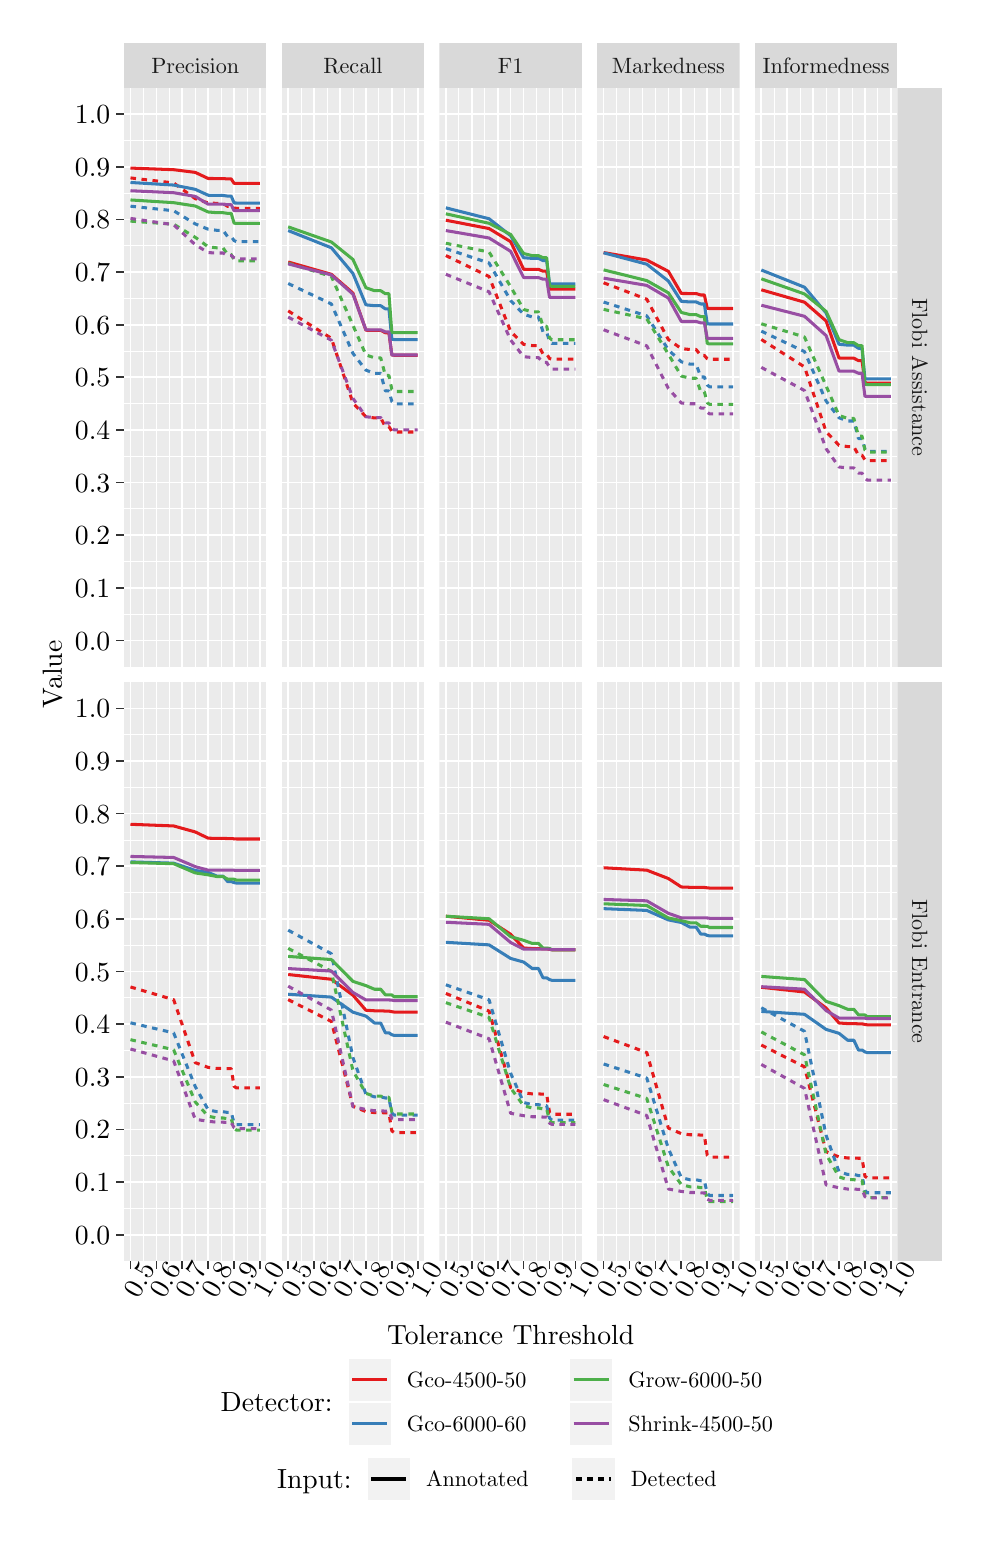
\begin{tikzpicture}[x=1pt,y=1pt]
\definecolor{fillColor}{RGB}{255,255,255}
\path[use as bounding box,fill=fillColor,fill opacity=0.00] (0,0) rectangle (336.00,539.88);
\begin{scope}
\path[clip] (  0.00,  0.00) rectangle (336.00,539.88);
\definecolor{drawColor}{RGB}{255,255,255}
\definecolor{fillColor}{RGB}{255,255,255}

\path[draw=drawColor,line width= 0.6pt,line join=round,line cap=round,fill=fillColor] (  0.00,  0.00) rectangle (336.00,539.88);
\end{scope}
\begin{scope}
\path[clip] ( 34.81,308.92) rectangle ( 86.29,518.13);
\definecolor{fillColor}{gray}{0.92}

\path[fill=fillColor] ( 34.81,308.92) rectangle ( 86.29,518.13);
\definecolor{drawColor}{RGB}{255,255,255}

\path[draw=drawColor,line width= 0.3pt,line join=round] ( 34.81,327.94) --
	( 86.29,327.94);

\path[draw=drawColor,line width= 0.3pt,line join=round] ( 34.81,346.96) --
	( 86.29,346.96);

\path[draw=drawColor,line width= 0.3pt,line join=round] ( 34.81,365.98) --
	( 86.29,365.98);

\path[draw=drawColor,line width= 0.3pt,line join=round] ( 34.81,385.00) --
	( 86.29,385.00);

\path[draw=drawColor,line width= 0.3pt,line join=round] ( 34.81,404.02) --
	( 86.29,404.02);

\path[draw=drawColor,line width= 0.3pt,line join=round] ( 34.81,423.03) --
	( 86.29,423.03);

\path[draw=drawColor,line width= 0.3pt,line join=round] ( 34.81,442.05) --
	( 86.29,442.05);

\path[draw=drawColor,line width= 0.3pt,line join=round] ( 34.81,461.07) --
	( 86.29,461.07);

\path[draw=drawColor,line width= 0.3pt,line join=round] ( 34.81,480.09) --
	( 86.29,480.09);

\path[draw=drawColor,line width= 0.3pt,line join=round] ( 34.81,499.11) --
	( 86.29,499.11);

\path[draw=drawColor,line width= 0.3pt,line join=round] ( 41.83,308.92) --
	( 41.83,518.13);

\path[draw=drawColor,line width= 0.3pt,line join=round] ( 46.51,308.92) --
	( 46.51,518.13);

\path[draw=drawColor,line width= 0.3pt,line join=round] ( 51.19,308.92) --
	( 51.19,518.13);

\path[draw=drawColor,line width= 0.3pt,line join=round] ( 55.87,308.92) --
	( 55.87,518.13);

\path[draw=drawColor,line width= 0.3pt,line join=round] ( 60.55,308.92) --
	( 60.55,518.13);

\path[draw=drawColor,line width= 0.3pt,line join=round] ( 69.91,308.92) --
	( 69.91,518.13);

\path[draw=drawColor,line width= 0.3pt,line join=round] ( 79.27,308.92) --
	( 79.27,518.13);

\path[draw=drawColor,line width= 0.6pt,line join=round] ( 34.81,318.43) --
	( 86.29,318.43);

\path[draw=drawColor,line width= 0.6pt,line join=round] ( 34.81,337.45) --
	( 86.29,337.45);

\path[draw=drawColor,line width= 0.6pt,line join=round] ( 34.81,356.47) --
	( 86.29,356.47);

\path[draw=drawColor,line width= 0.6pt,line join=round] ( 34.81,375.49) --
	( 86.29,375.49);

\path[draw=drawColor,line width= 0.6pt,line join=round] ( 34.81,394.51) --
	( 86.29,394.51);

\path[draw=drawColor,line width= 0.6pt,line join=round] ( 34.81,413.53) --
	( 86.29,413.53);

\path[draw=drawColor,line width= 0.6pt,line join=round] ( 34.81,432.54) --
	( 86.29,432.54);

\path[draw=drawColor,line width= 0.6pt,line join=round] ( 34.81,451.56) --
	( 86.29,451.56);

\path[draw=drawColor,line width= 0.6pt,line join=round] ( 34.81,470.58) --
	( 86.29,470.58);

\path[draw=drawColor,line width= 0.6pt,line join=round] ( 34.81,489.60) --
	( 86.29,489.60);

\path[draw=drawColor,line width= 0.6pt,line join=round] ( 34.81,508.62) --
	( 86.29,508.62);

\path[draw=drawColor,line width= 0.6pt,line join=round] ( 37.15,308.92) --
	( 37.15,518.13);

\path[draw=drawColor,line width= 0.6pt,line join=round] ( 46.51,308.92) --
	( 46.51,518.13);

\path[draw=drawColor,line width= 0.6pt,line join=round] ( 55.87,308.92) --
	( 55.87,518.13);

\path[draw=drawColor,line width= 0.6pt,line join=round] ( 65.23,308.92) --
	( 65.23,518.13);

\path[draw=drawColor,line width= 0.6pt,line join=round] ( 74.59,308.92) --
	( 74.59,518.13);

\path[draw=drawColor,line width= 0.6pt,line join=round] ( 83.95,308.92) --
	( 83.95,518.13);
\definecolor{drawColor}{RGB}{228,26,28}

\path[draw=drawColor,line width= 1.1pt,line join=round] ( 37.15,489.14) --
	( 52.75,488.55) --
	( 60.55,487.58) --
	( 65.23,485.37) --
	( 68.35,485.36) --
	( 70.58,485.36) --
	( 72.25,485.21) --
	( 73.55,485.21) --
	( 74.59,483.63) --
	( 75.44,483.60) --
	( 76.15,483.60) --
	( 83.94,483.60);

\path[draw=drawColor,line width= 1.1pt,dash pattern=on 2pt off 2pt ,line join=round] ( 37.15,485.58) --
	( 52.75,483.77) --
	( 60.55,478.08) --
	( 65.23,476.53) --
	( 68.35,476.38) --
	( 70.58,476.38) --
	( 72.25,475.30) --
	( 73.55,475.30) --
	( 74.59,474.69) --
	( 75.44,474.60) --
	( 76.15,474.60) --
	( 83.94,474.60);
\definecolor{drawColor}{RGB}{55,126,184}

\path[draw=drawColor,line width= 1.1pt,line join=round] ( 37.15,483.94) --
	( 52.75,483.00) --
	( 60.55,481.46) --
	( 65.23,479.32) --
	( 68.35,479.25) --
	( 70.58,479.25) --
	( 72.25,479.01) --
	( 73.55,479.01) --
	( 74.59,476.53) --
	( 75.44,476.51) --
	( 76.15,476.51) --
	( 83.94,476.51);

\path[draw=drawColor,line width= 1.1pt,dash pattern=on 2pt off 2pt ,line join=round] ( 37.15,475.37) --
	( 52.75,473.72) --
	( 60.55,468.97) --
	( 65.23,467.04) --
	( 68.35,466.65) --
	( 70.58,466.65) --
	( 72.25,464.39) --
	( 73.55,464.39) --
	( 74.59,462.92) --
	( 75.44,462.56) --
	( 76.15,462.56) --
	( 83.94,462.56);
\definecolor{drawColor}{RGB}{77,175,74}

\path[draw=drawColor,line width= 1.1pt,line join=round] ( 37.15,477.62) --
	( 52.75,476.64) --
	( 60.55,475.43) --
	( 65.23,473.27) --
	( 68.35,473.02) --
	( 70.58,473.02) --
	( 72.25,472.77) --
	( 73.55,472.77) --
	( 74.59,469.22) --
	( 75.44,469.17) --
	( 76.15,469.17) --
	( 83.94,469.17);

\path[draw=drawColor,line width= 1.1pt,dash pattern=on 2pt off 2pt ,line join=round] ( 37.15,469.97) --
	( 52.75,468.86) --
	( 60.55,464.13) --
	( 65.23,460.68) --
	( 68.35,460.32) --
	( 70.58,460.32) --
	( 72.25,457.95) --
	( 73.55,457.95) --
	( 74.59,455.93) --
	( 75.44,455.60) --
	( 76.15,455.60) --
	( 83.94,455.60);
\definecolor{drawColor}{RGB}{152,78,163}

\path[draw=drawColor,line width= 1.1pt,line join=round] ( 37.15,480.95) --
	( 52.75,480.24) --
	( 60.55,478.90) --
	( 65.23,476.08) --
	( 68.35,476.08) --
	( 70.58,476.08) --
	( 72.25,475.90) --
	( 73.55,475.90) --
	( 74.59,473.74) --
	( 75.44,473.74) --
	( 76.15,473.74) --
	( 83.94,473.74);

\path[draw=drawColor,line width= 1.1pt,dash pattern=on 2pt off 2pt ,line join=round] ( 37.15,470.95) --
	( 52.75,468.66) --
	( 60.55,461.45) --
	( 65.23,458.59) --
	( 68.35,458.45) --
	( 70.58,458.45) --
	( 72.25,457.57) --
	( 73.55,457.57) --
	( 74.59,456.70) --
	( 75.44,456.33) --
	( 76.15,456.33) --
	( 83.94,456.33);
\end{scope}
\begin{scope}
\path[clip] ( 34.81, 94.21) rectangle ( 86.29,303.42);
\definecolor{fillColor}{gray}{0.92}

\path[fill=fillColor] ( 34.81, 94.21) rectangle ( 86.29,303.42);
\definecolor{drawColor}{RGB}{255,255,255}

\path[draw=drawColor,line width= 0.3pt,line join=round] ( 34.81,113.23) --
	( 86.29,113.23);

\path[draw=drawColor,line width= 0.3pt,line join=round] ( 34.81,132.25) --
	( 86.29,132.25);

\path[draw=drawColor,line width= 0.3pt,line join=round] ( 34.81,151.27) --
	( 86.29,151.27);

\path[draw=drawColor,line width= 0.3pt,line join=round] ( 34.81,170.29) --
	( 86.29,170.29);

\path[draw=drawColor,line width= 0.3pt,line join=round] ( 34.81,189.30) --
	( 86.29,189.30);

\path[draw=drawColor,line width= 0.3pt,line join=round] ( 34.81,208.32) --
	( 86.29,208.32);

\path[draw=drawColor,line width= 0.3pt,line join=round] ( 34.81,227.34) --
	( 86.29,227.34);

\path[draw=drawColor,line width= 0.3pt,line join=round] ( 34.81,246.36) --
	( 86.29,246.36);

\path[draw=drawColor,line width= 0.3pt,line join=round] ( 34.81,265.38) --
	( 86.29,265.38);

\path[draw=drawColor,line width= 0.3pt,line join=round] ( 34.81,284.40) --
	( 86.29,284.40);

\path[draw=drawColor,line width= 0.3pt,line join=round] ( 41.83, 94.21) --
	( 41.83,303.42);

\path[draw=drawColor,line width= 0.3pt,line join=round] ( 46.51, 94.21) --
	( 46.51,303.42);

\path[draw=drawColor,line width= 0.3pt,line join=round] ( 51.19, 94.21) --
	( 51.19,303.42);

\path[draw=drawColor,line width= 0.3pt,line join=round] ( 55.87, 94.21) --
	( 55.87,303.42);

\path[draw=drawColor,line width= 0.3pt,line join=round] ( 60.55, 94.21) --
	( 60.55,303.42);

\path[draw=drawColor,line width= 0.3pt,line join=round] ( 69.91, 94.21) --
	( 69.91,303.42);

\path[draw=drawColor,line width= 0.3pt,line join=round] ( 79.27, 94.21) --
	( 79.27,303.42);

\path[draw=drawColor,line width= 0.6pt,line join=round] ( 34.81,103.72) --
	( 86.29,103.72);

\path[draw=drawColor,line width= 0.6pt,line join=round] ( 34.81,122.74) --
	( 86.29,122.74);

\path[draw=drawColor,line width= 0.6pt,line join=round] ( 34.81,141.76) --
	( 86.29,141.76);

\path[draw=drawColor,line width= 0.6pt,line join=round] ( 34.81,160.78) --
	( 86.29,160.78);

\path[draw=drawColor,line width= 0.6pt,line join=round] ( 34.81,179.79) --
	( 86.29,179.79);

\path[draw=drawColor,line width= 0.6pt,line join=round] ( 34.81,198.81) --
	( 86.29,198.81);

\path[draw=drawColor,line width= 0.6pt,line join=round] ( 34.81,217.83) --
	( 86.29,217.83);

\path[draw=drawColor,line width= 0.6pt,line join=round] ( 34.81,236.85) --
	( 86.29,236.85);

\path[draw=drawColor,line width= 0.6pt,line join=round] ( 34.81,255.87) --
	( 86.29,255.87);

\path[draw=drawColor,line width= 0.6pt,line join=round] ( 34.81,274.89) --
	( 86.29,274.89);

\path[draw=drawColor,line width= 0.6pt,line join=round] ( 34.81,293.91) --
	( 86.29,293.91);

\path[draw=drawColor,line width= 0.6pt,line join=round] ( 37.15, 94.21) --
	( 37.15,303.42);

\path[draw=drawColor,line width= 0.6pt,line join=round] ( 46.51, 94.21) --
	( 46.51,303.42);

\path[draw=drawColor,line width= 0.6pt,line join=round] ( 55.87, 94.21) --
	( 55.87,303.42);

\path[draw=drawColor,line width= 0.6pt,line join=round] ( 65.23, 94.21) --
	( 65.23,303.42);

\path[draw=drawColor,line width= 0.6pt,line join=round] ( 74.59, 94.21) --
	( 74.59,303.42);

\path[draw=drawColor,line width= 0.6pt,line join=round] ( 83.95, 94.21) --
	( 83.95,303.42);
\definecolor{drawColor}{RGB}{228,26,28}

\path[draw=drawColor,line width= 1.1pt,line join=round] ( 37.15,252.02) --
	( 52.75,251.42) --
	( 60.55,249.25) --
	( 65.23,247.00) --
	( 68.35,246.91) --
	( 70.58,246.91) --
	( 72.25,246.87) --
	( 73.55,246.87) --
	( 74.59,246.77) --
	( 75.44,246.71) --
	( 76.15,246.71) --
	( 83.94,246.71);

\path[draw=drawColor,line width= 1.1pt,dash pattern=on 2pt off 2pt ,line join=round] ( 37.15,193.24) --
	( 52.75,188.64) --
	( 60.55,165.89) --
	( 65.23,164.17) --
	( 68.35,163.81) --
	( 70.58,163.81) --
	( 72.25,163.72) --
	( 73.55,163.72) --
	( 74.59,157.34) --
	( 75.44,156.74) --
	( 76.15,156.74) --
	( 83.94,156.74);
\definecolor{drawColor}{RGB}{55,126,184}

\path[draw=drawColor,line width= 1.1pt,line join=round] ( 37.15,238.44) --
	( 52.75,237.97) --
	( 60.55,235.34) --
	( 65.23,234.62) --
	( 68.35,233.30) --
	( 70.58,233.30) --
	( 72.25,231.32) --
	( 73.55,231.32) --
	( 74.59,230.93) --
	( 75.44,230.78) --
	( 76.15,230.78) --
	( 83.94,230.78);

\path[draw=drawColor,line width= 1.1pt,dash pattern=on 2pt off 2pt ,line join=round] ( 37.15,180.28) --
	( 52.75,176.64) --
	( 60.55,157.26) --
	( 65.23,148.83) --
	( 68.35,148.17) --
	( 70.58,148.17) --
	( 72.25,147.89) --
	( 73.55,147.89) --
	( 74.59,144.10) --
	( 75.44,143.51) --
	( 76.15,143.51) --
	( 83.94,143.51);
\definecolor{drawColor}{RGB}{77,175,74}

\path[draw=drawColor,line width= 1.1pt,line join=round] ( 37.15,238.22) --
	( 52.75,237.77) --
	( 60.55,234.45) --
	( 65.23,233.75) --
	( 68.35,233.14) --
	( 70.58,233.14) --
	( 72.25,232.20) --
	( 73.55,232.20) --
	( 74.59,232.17) --
	( 75.44,231.86) --
	( 76.15,231.86) --
	( 83.94,231.86);

\path[draw=drawColor,line width= 1.1pt,dash pattern=on 2pt off 2pt ,line join=round] ( 37.15,174.19) --
	( 52.75,170.54) --
	( 60.55,151.68) --
	( 65.23,146.54) --
	( 68.35,145.89) --
	( 70.58,145.89) --
	( 72.25,145.62) --
	( 73.55,145.62) --
	( 74.59,142.10) --
	( 75.44,141.53) --
	( 76.15,141.53) --
	( 83.94,141.53);
\definecolor{drawColor}{RGB}{152,78,163}

\path[draw=drawColor,line width= 1.1pt,line join=round] ( 37.15,240.40) --
	( 52.75,240.03) --
	( 60.55,236.71) --
	( 65.23,235.44) --
	( 68.35,235.44) --
	( 70.58,235.44) --
	( 72.25,235.44) --
	( 73.55,235.44) --
	( 74.59,235.42) --
	( 75.44,235.33) --
	( 76.15,235.33) --
	( 83.94,235.33);

\path[draw=drawColor,line width= 1.1pt,dash pattern=on 2pt off 2pt ,line join=round] ( 37.15,170.82) --
	( 52.75,166.50) --
	( 60.55,145.42) --
	( 65.23,144.70) --
	( 68.35,144.37) --
	( 70.58,144.37) --
	( 72.25,144.28) --
	( 73.55,144.28) --
	( 74.59,142.38) --
	( 75.44,142.04) --
	( 76.15,142.04) --
	( 83.94,142.04);
\end{scope}
\begin{scope}
\path[clip] ( 91.79,308.92) rectangle (143.28,518.13);
\definecolor{fillColor}{gray}{0.92}

\path[fill=fillColor] ( 91.79,308.92) rectangle (143.28,518.13);
\definecolor{drawColor}{RGB}{255,255,255}

\path[draw=drawColor,line width= 0.3pt,line join=round] ( 91.79,327.94) --
	(143.28,327.94);

\path[draw=drawColor,line width= 0.3pt,line join=round] ( 91.79,346.96) --
	(143.28,346.96);

\path[draw=drawColor,line width= 0.3pt,line join=round] ( 91.79,365.98) --
	(143.28,365.98);

\path[draw=drawColor,line width= 0.3pt,line join=round] ( 91.79,385.00) --
	(143.28,385.00);

\path[draw=drawColor,line width= 0.3pt,line join=round] ( 91.79,404.02) --
	(143.28,404.02);

\path[draw=drawColor,line width= 0.3pt,line join=round] ( 91.79,423.03) --
	(143.28,423.03);

\path[draw=drawColor,line width= 0.3pt,line join=round] ( 91.79,442.05) --
	(143.28,442.05);

\path[draw=drawColor,line width= 0.3pt,line join=round] ( 91.79,461.07) --
	(143.28,461.07);

\path[draw=drawColor,line width= 0.3pt,line join=round] ( 91.79,480.09) --
	(143.28,480.09);

\path[draw=drawColor,line width= 0.3pt,line join=round] ( 91.79,499.11) --
	(143.28,499.11);

\path[draw=drawColor,line width= 0.3pt,line join=round] ( 98.82,308.92) --
	( 98.82,518.13);

\path[draw=drawColor,line width= 0.3pt,line join=round] (103.50,308.92) --
	(103.50,518.13);

\path[draw=drawColor,line width= 0.3pt,line join=round] (108.18,308.92) --
	(108.18,518.13);

\path[draw=drawColor,line width= 0.3pt,line join=round] (112.86,308.92) --
	(112.86,518.13);

\path[draw=drawColor,line width= 0.3pt,line join=round] (117.54,308.92) --
	(117.54,518.13);

\path[draw=drawColor,line width= 0.3pt,line join=round] (126.90,308.92) --
	(126.90,518.13);

\path[draw=drawColor,line width= 0.3pt,line join=round] (136.26,308.92) --
	(136.26,518.13);

\path[draw=drawColor,line width= 0.6pt,line join=round] ( 91.79,318.43) --
	(143.28,318.43);

\path[draw=drawColor,line width= 0.6pt,line join=round] ( 91.79,337.45) --
	(143.28,337.45);

\path[draw=drawColor,line width= 0.6pt,line join=round] ( 91.79,356.47) --
	(143.28,356.47);

\path[draw=drawColor,line width= 0.6pt,line join=round] ( 91.79,375.49) --
	(143.28,375.49);

\path[draw=drawColor,line width= 0.6pt,line join=round] ( 91.79,394.51) --
	(143.28,394.51);

\path[draw=drawColor,line width= 0.6pt,line join=round] ( 91.79,413.53) --
	(143.28,413.53);

\path[draw=drawColor,line width= 0.6pt,line join=round] ( 91.79,432.54) --
	(143.28,432.54);

\path[draw=drawColor,line width= 0.6pt,line join=round] ( 91.79,451.56) --
	(143.28,451.56);

\path[draw=drawColor,line width= 0.6pt,line join=round] ( 91.79,470.58) --
	(143.28,470.58);

\path[draw=drawColor,line width= 0.6pt,line join=round] ( 91.79,489.60) --
	(143.28,489.60);

\path[draw=drawColor,line width= 0.6pt,line join=round] ( 91.79,508.62) --
	(143.28,508.62);

\path[draw=drawColor,line width= 0.6pt,line join=round] ( 94.13,308.92) --
	( 94.13,518.13);

\path[draw=drawColor,line width= 0.6pt,line join=round] (103.50,308.92) --
	(103.50,518.13);

\path[draw=drawColor,line width= 0.6pt,line join=round] (112.86,308.92) --
	(112.86,518.13);

\path[draw=drawColor,line width= 0.6pt,line join=round] (122.22,308.92) --
	(122.22,518.13);

\path[draw=drawColor,line width= 0.6pt,line join=round] (131.58,308.92) --
	(131.58,518.13);

\path[draw=drawColor,line width= 0.6pt,line join=round] (140.94,308.92) --
	(140.94,518.13);
\definecolor{drawColor}{RGB}{228,26,28}

\path[draw=drawColor,line width= 1.1pt,line join=round] ( 94.13,455.21) --
	(109.74,450.75) --
	(117.54,443.96) --
	(122.22,430.55) --
	(125.34,430.50) --
	(127.57,430.50) --
	(129.24,429.64) --
	(130.54,429.64) --
	(131.58,421.65) --
	(132.43,421.50) --
	(133.14,421.50) --
	(140.93,421.50);

\path[draw=drawColor,line width= 1.1pt,dash pattern=on 2pt off 2pt ,line join=round] ( 94.13,437.54) --
	(109.74,427.62) --
	(117.54,404.24) --
	(122.22,399.30) --
	(125.34,398.84) --
	(127.57,398.84) --
	(129.24,395.70) --
	(130.54,395.70) --
	(131.58,394.03) --
	(132.43,393.77) --
	(133.14,393.77) --
	(140.93,393.77);
\definecolor{drawColor}{RGB}{55,126,184}

\path[draw=drawColor,line width= 1.1pt,line join=round] ( 94.13,466.56) --
	(109.74,460.34) --
	(117.54,451.04) --
	(122.22,439.72) --
	(125.34,439.41) --
	(127.57,439.41) --
	(129.24,438.26) --
	(130.54,438.26) --
	(131.58,427.28) --
	(132.43,427.18) --
	(133.14,427.18) --
	(140.93,427.18);

\path[draw=drawColor,line width= 1.1pt,dash pattern=on 2pt off 2pt ,line join=round] ( 94.13,447.43) --
	(109.74,440.04) --
	(117.54,422.18) --
	(122.22,416.12) --
	(125.34,414.95) --
	(127.57,414.95) --
	(129.24,408.62) --
	(130.54,408.62) --
	(131.58,404.82) --
	(132.43,403.94) --
	(133.14,403.94) --
	(140.93,403.94);
\definecolor{drawColor}{RGB}{77,175,74}

\path[draw=drawColor,line width= 1.1pt,line join=round] ( 94.13,467.90) --
	(109.74,462.42) --
	(117.54,456.12) --
	(122.22,445.91) --
	(125.34,444.82) --
	(127.57,444.82) --
	(129.24,443.74) --
	(130.54,443.74) --
	(131.58,429.84) --
	(132.43,429.65) --
	(133.14,429.65) --
	(140.93,429.65);

\path[draw=drawColor,line width= 1.1pt,dash pattern=on 2pt off 2pt ,line join=round] ( 94.13,454.77) --
	(109.74,449.99) --
	(117.54,432.33) --
	(122.22,421.63) --
	(125.34,420.58) --
	(127.57,420.58) --
	(129.24,414.19) --
	(130.54,414.19) --
	(131.58,409.18) --
	(132.43,408.41) --
	(133.14,408.41) --
	(140.93,408.41);
\definecolor{drawColor}{RGB}{152,78,163}

\path[draw=drawColor,line width= 1.1pt,line join=round] ( 94.13,454.52) --
	(109.74,450.53) --
	(117.54,443.56) --
	(122.22,430.69) --
	(125.34,430.69) --
	(127.57,430.69) --
	(129.24,429.94) --
	(130.54,429.94) --
	(131.58,421.59) --
	(132.43,421.59) --
	(133.14,421.59) --
	(140.93,421.59);

\path[draw=drawColor,line width= 1.1pt,dash pattern=on 2pt off 2pt ,line join=round] ( 94.13,435.29) --
	(109.74,426.93) --
	(117.54,405.93) --
	(122.22,399.28) --
	(125.34,398.96) --
	(127.57,398.96) --
	(129.24,397.08) --
	(130.54,397.08) --
	(131.58,395.28) --
	(132.43,394.54) --
	(133.14,394.54) --
	(140.93,394.54);
\end{scope}
\begin{scope}
\path[clip] ( 91.79, 94.21) rectangle (143.28,303.42);
\definecolor{fillColor}{gray}{0.92}

\path[fill=fillColor] ( 91.79, 94.21) rectangle (143.28,303.42);
\definecolor{drawColor}{RGB}{255,255,255}

\path[draw=drawColor,line width= 0.3pt,line join=round] ( 91.79,113.23) --
	(143.28,113.23);

\path[draw=drawColor,line width= 0.3pt,line join=round] ( 91.79,132.25) --
	(143.28,132.25);

\path[draw=drawColor,line width= 0.3pt,line join=round] ( 91.79,151.27) --
	(143.28,151.27);

\path[draw=drawColor,line width= 0.3pt,line join=round] ( 91.79,170.29) --
	(143.28,170.29);

\path[draw=drawColor,line width= 0.3pt,line join=round] ( 91.79,189.30) --
	(143.28,189.30);

\path[draw=drawColor,line width= 0.3pt,line join=round] ( 91.79,208.32) --
	(143.28,208.32);

\path[draw=drawColor,line width= 0.3pt,line join=round] ( 91.79,227.34) --
	(143.28,227.34);

\path[draw=drawColor,line width= 0.3pt,line join=round] ( 91.79,246.36) --
	(143.28,246.36);

\path[draw=drawColor,line width= 0.3pt,line join=round] ( 91.79,265.38) --
	(143.28,265.38);

\path[draw=drawColor,line width= 0.3pt,line join=round] ( 91.79,284.40) --
	(143.28,284.40);

\path[draw=drawColor,line width= 0.3pt,line join=round] ( 98.82, 94.21) --
	( 98.82,303.42);

\path[draw=drawColor,line width= 0.3pt,line join=round] (103.50, 94.21) --
	(103.50,303.42);

\path[draw=drawColor,line width= 0.3pt,line join=round] (108.18, 94.21) --
	(108.18,303.42);

\path[draw=drawColor,line width= 0.3pt,line join=round] (112.86, 94.21) --
	(112.86,303.42);

\path[draw=drawColor,line width= 0.3pt,line join=round] (117.54, 94.21) --
	(117.54,303.42);

\path[draw=drawColor,line width= 0.3pt,line join=round] (126.90, 94.21) --
	(126.90,303.42);

\path[draw=drawColor,line width= 0.3pt,line join=round] (136.26, 94.21) --
	(136.26,303.42);

\path[draw=drawColor,line width= 0.6pt,line join=round] ( 91.79,103.72) --
	(143.28,103.72);

\path[draw=drawColor,line width= 0.6pt,line join=round] ( 91.79,122.74) --
	(143.28,122.74);

\path[draw=drawColor,line width= 0.6pt,line join=round] ( 91.79,141.76) --
	(143.28,141.76);

\path[draw=drawColor,line width= 0.6pt,line join=round] ( 91.79,160.78) --
	(143.28,160.78);

\path[draw=drawColor,line width= 0.6pt,line join=round] ( 91.79,179.79) --
	(143.28,179.79);

\path[draw=drawColor,line width= 0.6pt,line join=round] ( 91.79,198.81) --
	(143.28,198.81);

\path[draw=drawColor,line width= 0.6pt,line join=round] ( 91.79,217.83) --
	(143.28,217.83);

\path[draw=drawColor,line width= 0.6pt,line join=round] ( 91.79,236.85) --
	(143.28,236.85);

\path[draw=drawColor,line width= 0.6pt,line join=round] ( 91.79,255.87) --
	(143.28,255.87);

\path[draw=drawColor,line width= 0.6pt,line join=round] ( 91.79,274.89) --
	(143.28,274.89);

\path[draw=drawColor,line width= 0.6pt,line join=round] ( 91.79,293.91) --
	(143.28,293.91);

\path[draw=drawColor,line width= 0.6pt,line join=round] ( 94.13, 94.21) --
	( 94.13,303.42);

\path[draw=drawColor,line width= 0.6pt,line join=round] (103.50, 94.21) --
	(103.50,303.42);

\path[draw=drawColor,line width= 0.6pt,line join=round] (112.86, 94.21) --
	(112.86,303.42);

\path[draw=drawColor,line width= 0.6pt,line join=round] (122.22, 94.21) --
	(122.22,303.42);

\path[draw=drawColor,line width= 0.6pt,line join=round] (131.58, 94.21) --
	(131.58,303.42);

\path[draw=drawColor,line width= 0.6pt,line join=round] (140.94, 94.21) --
	(140.94,303.42);
\definecolor{drawColor}{RGB}{228,26,28}

\path[draw=drawColor,line width= 1.1pt,line join=round] ( 94.13,197.74) --
	(109.74,196.02) --
	(117.54,190.26) --
	(122.22,184.83) --
	(125.34,184.63) --
	(127.57,184.63) --
	(129.24,184.52) --
	(130.54,184.52) --
	(131.58,184.30) --
	(132.43,184.17) --
	(133.14,184.17) --
	(140.93,184.17);

\path[draw=drawColor,line width= 1.1pt,dash pattern=on 2pt off 2pt ,line join=round] ( 94.13,188.66) --
	(109.74,180.78) --
	(117.54,150.11) --
	(122.22,148.22) --
	(125.34,147.84) --
	(127.57,147.84) --
	(129.24,147.74) --
	(130.54,147.74) --
	(131.58,141.23) --
	(132.43,140.64) --
	(133.14,140.64) --
	(140.93,140.64);
\definecolor{drawColor}{RGB}{55,126,184}

\path[draw=drawColor,line width= 1.1pt,line join=round] ( 94.13,190.61) --
	(109.74,189.58) --
	(117.54,184.12) --
	(122.22,182.71) --
	(125.34,180.20) --
	(127.57,180.20) --
	(129.24,176.67) --
	(130.54,176.67) --
	(131.58,175.98) --
	(132.43,175.73) --
	(133.14,175.73) --
	(140.93,175.73);

\path[draw=drawColor,line width= 1.1pt,dash pattern=on 2pt off 2pt ,line join=round] ( 94.13,213.76) --
	(109.74,205.26) --
	(117.54,167.70) --
	(122.22,154.50) --
	(125.34,153.53) --
	(127.57,153.53) --
	(129.24,153.12) --
	(130.54,153.12) --
	(131.58,147.74) --
	(132.43,146.92) --
	(133.14,146.92) --
	(140.93,146.92);
\definecolor{drawColor}{RGB}{77,175,74}

\path[draw=drawColor,line width= 1.1pt,line join=round] ( 94.13,204.28) --
	(109.74,203.15) --
	(117.54,195.26) --
	(122.22,193.72) --
	(125.34,192.41) --
	(127.57,192.41) --
	(129.24,190.41) --
	(130.54,190.41) --
	(131.58,190.36) --
	(132.43,189.70) --
	(133.14,189.70) --
	(140.93,189.70);

\path[draw=drawColor,line width= 1.1pt,dash pattern=on 2pt off 2pt ,line join=round] ( 94.13,207.18) --
	(109.74,198.90) --
	(117.54,162.98) --
	(122.22,154.78) --
	(125.34,153.79) --
	(127.57,153.79) --
	(129.24,153.38) --
	(130.54,153.38) --
	(131.58,148.14) --
	(132.43,147.33) --
	(133.14,147.33) --
	(140.93,147.33);
\definecolor{drawColor}{RGB}{152,78,163}

\path[draw=drawColor,line width= 1.1pt,line join=round] ( 94.13,199.89) --
	(109.74,198.98) --
	(117.54,191.25) --
	(122.22,188.54) --
	(125.34,188.54) --
	(127.57,188.54) --
	(129.24,188.54) --
	(130.54,188.54) --
	(131.58,188.49) --
	(132.43,188.32) --
	(133.14,188.32) --
	(140.93,188.32);

\path[draw=drawColor,line width= 1.1pt,dash pattern=on 2pt off 2pt ,line join=round] ( 94.13,193.52) --
	(109.74,184.89) --
	(117.54,149.98) --
	(122.22,148.96) --
	(125.34,148.50) --
	(127.57,148.50) --
	(129.24,148.37) --
	(130.54,148.37) --
	(131.58,145.74) --
	(132.43,145.28) --
	(133.14,145.28) --
	(140.93,145.28);
\end{scope}
\begin{scope}
\path[clip] (148.78,308.92) rectangle (200.27,518.13);
\definecolor{fillColor}{gray}{0.92}

\path[fill=fillColor] (148.78,308.92) rectangle (200.27,518.13);
\definecolor{drawColor}{RGB}{255,255,255}

\path[draw=drawColor,line width= 0.3pt,line join=round] (148.78,327.94) --
	(200.27,327.94);

\path[draw=drawColor,line width= 0.3pt,line join=round] (148.78,346.96) --
	(200.27,346.96);

\path[draw=drawColor,line width= 0.3pt,line join=round] (148.78,365.98) --
	(200.27,365.98);

\path[draw=drawColor,line width= 0.3pt,line join=round] (148.78,385.00) --
	(200.27,385.00);

\path[draw=drawColor,line width= 0.3pt,line join=round] (148.78,404.02) --
	(200.27,404.02);

\path[draw=drawColor,line width= 0.3pt,line join=round] (148.78,423.03) --
	(200.27,423.03);

\path[draw=drawColor,line width= 0.3pt,line join=round] (148.78,442.05) --
	(200.27,442.05);

\path[draw=drawColor,line width= 0.3pt,line join=round] (148.78,461.07) --
	(200.27,461.07);

\path[draw=drawColor,line width= 0.3pt,line join=round] (148.78,480.09) --
	(200.27,480.09);

\path[draw=drawColor,line width= 0.3pt,line join=round] (148.78,499.11) --
	(200.27,499.11);

\path[draw=drawColor,line width= 0.3pt,line join=round] (155.80,308.92) --
	(155.80,518.13);

\path[draw=drawColor,line width= 0.3pt,line join=round] (160.48,308.92) --
	(160.48,518.13);

\path[draw=drawColor,line width= 0.3pt,line join=round] (165.16,308.92) --
	(165.16,518.13);

\path[draw=drawColor,line width= 0.3pt,line join=round] (169.85,308.92) --
	(169.85,518.13);

\path[draw=drawColor,line width= 0.3pt,line join=round] (174.53,308.92) --
	(174.53,518.13);

\path[draw=drawColor,line width= 0.3pt,line join=round] (183.89,308.92) --
	(183.89,518.13);

\path[draw=drawColor,line width= 0.3pt,line join=round] (193.25,308.92) --
	(193.25,518.13);

\path[draw=drawColor,line width= 0.6pt,line join=round] (148.78,318.43) --
	(200.27,318.43);

\path[draw=drawColor,line width= 0.6pt,line join=round] (148.78,337.45) --
	(200.27,337.45);

\path[draw=drawColor,line width= 0.6pt,line join=round] (148.78,356.47) --
	(200.27,356.47);

\path[draw=drawColor,line width= 0.6pt,line join=round] (148.78,375.49) --
	(200.27,375.49);

\path[draw=drawColor,line width= 0.6pt,line join=round] (148.78,394.51) --
	(200.27,394.51);

\path[draw=drawColor,line width= 0.6pt,line join=round] (148.78,413.53) --
	(200.27,413.53);

\path[draw=drawColor,line width= 0.6pt,line join=round] (148.78,432.54) --
	(200.27,432.54);

\path[draw=drawColor,line width= 0.6pt,line join=round] (148.78,451.56) --
	(200.27,451.56);

\path[draw=drawColor,line width= 0.6pt,line join=round] (148.78,470.58) --
	(200.27,470.58);

\path[draw=drawColor,line width= 0.6pt,line join=round] (148.78,489.60) --
	(200.27,489.60);

\path[draw=drawColor,line width= 0.6pt,line join=round] (148.78,508.62) --
	(200.27,508.62);

\path[draw=drawColor,line width= 0.6pt,line join=round] (151.12,308.92) --
	(151.12,518.13);

\path[draw=drawColor,line width= 0.6pt,line join=round] (160.48,308.92) --
	(160.48,518.13);

\path[draw=drawColor,line width= 0.6pt,line join=round] (169.85,308.92) --
	(169.85,518.13);

\path[draw=drawColor,line width= 0.6pt,line join=round] (179.21,308.92) --
	(179.21,518.13);

\path[draw=drawColor,line width= 0.6pt,line join=round] (188.57,308.92) --
	(188.57,518.13);

\path[draw=drawColor,line width= 0.6pt,line join=round] (197.93,308.92) --
	(197.93,518.13);
\definecolor{drawColor}{RGB}{228,26,28}

\path[draw=drawColor,line width= 1.1pt,line join=round] (151.12,470.30) --
	(166.72,467.28) --
	(174.53,462.54) --
	(179.21,452.58) --
	(182.33,452.54) --
	(184.56,452.54) --
	(186.23,451.87) --
	(187.53,451.87) --
	(188.57,445.48) --
	(189.42,445.37) --
	(190.13,445.37) --
	(197.92,445.37);

\path[draw=drawColor,line width= 1.1pt,dash pattern=on 2pt off 2pt ,line join=round] (151.12,457.53) --
	(166.72,449.95) --
	(174.53,430.06) --
	(179.21,425.44) --
	(182.33,425.00) --
	(184.56,425.00) --
	(186.23,421.97) --
	(187.53,421.97) --
	(188.57,420.33) --
	(189.42,420.08) --
	(190.13,420.08) --
	(197.92,420.08);
\definecolor{drawColor}{RGB}{55,126,184}

\path[draw=drawColor,line width= 1.1pt,line join=round] (151.12,474.77) --
	(166.72,470.83) --
	(174.53,464.69) --
	(179.21,456.74) --
	(182.33,456.51) --
	(184.56,456.51) --
	(186.23,455.68) --
	(187.53,455.68) --
	(188.57,447.36) --
	(189.42,447.29) --
	(190.13,447.29) --
	(197.92,447.29);

\path[draw=drawColor,line width= 1.1pt,dash pattern=on 2pt off 2pt ,line join=round] (151.12,460.03) --
	(166.72,454.83) --
	(174.53,441.27) --
	(179.21,436.31) --
	(182.33,435.34) --
	(184.56,435.34) --
	(186.23,429.92) --
	(187.53,429.92) --
	(188.57,426.56) --
	(189.42,425.77) --
	(190.13,425.77) --
	(197.92,425.77);
\definecolor{drawColor}{RGB}{77,175,74}

\path[draw=drawColor,line width= 1.1pt,line join=round] (151.12,472.61) --
	(166.72,469.19) --
	(174.53,465.14) --
	(179.21,458.26) --
	(182.33,457.50) --
	(184.56,457.50) --
	(186.23,456.75) --
	(187.53,456.75) --
	(188.57,446.57) --
	(189.42,446.42) --
	(190.13,446.42) --
	(197.92,446.42);

\path[draw=drawColor,line width= 1.1pt,dash pattern=on 2pt off 2pt ,line join=round] (151.12,461.97) --
	(166.72,458.79) --
	(174.53,446.28) --
	(179.21,438.05) --
	(182.33,437.21) --
	(184.56,437.21) --
	(186.23,432.00) --
	(187.53,432.00) --
	(188.57,427.77) --
	(189.42,427.10) --
	(190.13,427.10) --
	(197.92,427.10);
\definecolor{drawColor}{RGB}{152,78,163}

\path[draw=drawColor,line width= 1.1pt,line join=round] (151.12,466.56) --
	(166.72,463.88) --
	(174.53,459.05) --
	(179.21,449.57) --
	(182.33,449.57) --
	(184.56,449.57) --
	(186.23,448.99) --
	(187.53,448.99) --
	(188.57,442.40) --
	(189.42,442.40) --
	(190.13,442.40) --
	(197.92,442.40);

\path[draw=drawColor,line width= 1.1pt,dash pattern=on 2pt off 2pt ,line join=round] (151.12,450.76) --
	(166.72,444.43) --
	(174.53,427.00) --
	(179.21,420.98) --
	(182.33,420.68) --
	(184.56,420.68) --
	(186.23,418.92) --
	(187.53,418.92) --
	(188.57,417.22) --
	(189.42,416.51) --
	(190.13,416.51) --
	(197.92,416.51);
\end{scope}
\begin{scope}
\path[clip] (148.78, 94.21) rectangle (200.27,303.42);
\definecolor{fillColor}{gray}{0.92}

\path[fill=fillColor] (148.78, 94.21) rectangle (200.27,303.42);
\definecolor{drawColor}{RGB}{255,255,255}

\path[draw=drawColor,line width= 0.3pt,line join=round] (148.78,113.23) --
	(200.27,113.23);

\path[draw=drawColor,line width= 0.3pt,line join=round] (148.78,132.25) --
	(200.27,132.25);

\path[draw=drawColor,line width= 0.3pt,line join=round] (148.78,151.27) --
	(200.27,151.27);

\path[draw=drawColor,line width= 0.3pt,line join=round] (148.78,170.29) --
	(200.27,170.29);

\path[draw=drawColor,line width= 0.3pt,line join=round] (148.78,189.30) --
	(200.27,189.30);

\path[draw=drawColor,line width= 0.3pt,line join=round] (148.78,208.32) --
	(200.27,208.32);

\path[draw=drawColor,line width= 0.3pt,line join=round] (148.78,227.34) --
	(200.27,227.34);

\path[draw=drawColor,line width= 0.3pt,line join=round] (148.78,246.36) --
	(200.27,246.36);

\path[draw=drawColor,line width= 0.3pt,line join=round] (148.78,265.38) --
	(200.27,265.38);

\path[draw=drawColor,line width= 0.3pt,line join=round] (148.78,284.40) --
	(200.27,284.40);

\path[draw=drawColor,line width= 0.3pt,line join=round] (155.80, 94.21) --
	(155.80,303.42);

\path[draw=drawColor,line width= 0.3pt,line join=round] (160.48, 94.21) --
	(160.48,303.42);

\path[draw=drawColor,line width= 0.3pt,line join=round] (165.16, 94.21) --
	(165.16,303.42);

\path[draw=drawColor,line width= 0.3pt,line join=round] (169.85, 94.21) --
	(169.85,303.42);

\path[draw=drawColor,line width= 0.3pt,line join=round] (174.53, 94.21) --
	(174.53,303.42);

\path[draw=drawColor,line width= 0.3pt,line join=round] (183.89, 94.21) --
	(183.89,303.42);

\path[draw=drawColor,line width= 0.3pt,line join=round] (193.25, 94.21) --
	(193.25,303.42);

\path[draw=drawColor,line width= 0.6pt,line join=round] (148.78,103.72) --
	(200.27,103.72);

\path[draw=drawColor,line width= 0.6pt,line join=round] (148.78,122.74) --
	(200.27,122.74);

\path[draw=drawColor,line width= 0.6pt,line join=round] (148.78,141.76) --
	(200.27,141.76);

\path[draw=drawColor,line width= 0.6pt,line join=round] (148.78,160.78) --
	(200.27,160.78);

\path[draw=drawColor,line width= 0.6pt,line join=round] (148.78,179.79) --
	(200.27,179.79);

\path[draw=drawColor,line width= 0.6pt,line join=round] (148.78,198.81) --
	(200.27,198.81);

\path[draw=drawColor,line width= 0.6pt,line join=round] (148.78,217.83) --
	(200.27,217.83);

\path[draw=drawColor,line width= 0.6pt,line join=round] (148.78,236.85) --
	(200.27,236.85);

\path[draw=drawColor,line width= 0.6pt,line join=round] (148.78,255.87) --
	(200.27,255.87);

\path[draw=drawColor,line width= 0.6pt,line join=round] (148.78,274.89) --
	(200.27,274.89);

\path[draw=drawColor,line width= 0.6pt,line join=round] (148.78,293.91) --
	(200.27,293.91);

\path[draw=drawColor,line width= 0.6pt,line join=round] (151.12, 94.21) --
	(151.12,303.42);

\path[draw=drawColor,line width= 0.6pt,line join=round] (160.48, 94.21) --
	(160.48,303.42);

\path[draw=drawColor,line width= 0.6pt,line join=round] (169.85, 94.21) --
	(169.85,303.42);

\path[draw=drawColor,line width= 0.6pt,line join=round] (179.21, 94.21) --
	(179.21,303.42);

\path[draw=drawColor,line width= 0.6pt,line join=round] (188.57, 94.21) --
	(188.57,303.42);

\path[draw=drawColor,line width= 0.6pt,line join=round] (197.93, 94.21) --
	(197.93,303.42);
\definecolor{drawColor}{RGB}{228,26,28}

\path[draw=drawColor,line width= 1.1pt,line join=round] (151.12,218.80) --
	(166.72,217.33) --
	(174.53,212.26) --
	(179.21,207.30) --
	(182.33,207.11) --
	(184.56,207.11) --
	(186.23,207.02) --
	(187.53,207.02) --
	(188.57,206.81) --
	(189.42,206.69) --
	(190.13,206.69) --
	(197.92,206.69);

\path[draw=drawColor,line width= 1.1pt,dash pattern=on 2pt off 2pt ,line join=round] (151.12,190.89) --
	(166.72,184.52) --
	(174.53,156.86) --
	(179.21,154.98) --
	(182.33,154.60) --
	(184.56,154.60) --
	(186.23,154.50) --
	(187.53,154.50) --
	(188.57,147.86) --
	(189.42,147.25) --
	(190.13,147.25) --
	(197.92,147.25);
\definecolor{drawColor}{RGB}{55,126,184}

\path[draw=drawColor,line width= 1.1pt,line join=round] (151.12,209.37) --
	(166.72,208.45) --
	(174.53,203.54) --
	(179.21,202.24) --
	(182.33,199.91) --
	(184.56,199.91) --
	(186.23,196.55) --
	(187.53,196.55) --
	(188.57,195.89) --
	(189.42,195.64) --
	(190.13,195.64) --
	(197.92,195.64);

\path[draw=drawColor,line width= 1.1pt,dash pattern=on 2pt off 2pt ,line join=round] (151.12,194.02) --
	(166.72,188.60) --
	(174.53,162.02) --
	(179.21,151.50) --
	(182.33,150.70) --
	(184.56,150.70) --
	(186.23,150.36) --
	(187.53,150.36) --
	(188.57,145.84) --
	(189.42,145.14) --
	(190.13,145.14) --
	(197.92,145.14);
\definecolor{drawColor}{RGB}{77,175,74}

\path[draw=drawColor,line width= 1.1pt,line join=round] (151.12,218.80) --
	(166.72,217.89) --
	(174.53,211.40) --
	(179.21,210.10) --
	(182.33,208.97) --
	(184.56,208.97) --
	(186.23,207.25) --
	(187.53,207.25) --
	(188.57,207.20) --
	(189.42,206.63) --
	(190.13,206.63) --
	(197.92,206.63);

\path[draw=drawColor,line width= 1.1pt,dash pattern=on 2pt off 2pt ,line join=round] (151.12,187.56) --
	(166.72,182.24) --
	(174.53,156.73) --
	(179.21,150.30) --
	(182.33,149.50) --
	(184.56,149.50) --
	(186.23,149.17) --
	(187.53,149.17) --
	(188.57,144.90) --
	(189.42,144.22) --
	(190.13,144.22) --
	(197.92,144.22);
\definecolor{drawColor}{RGB}{152,78,163}

\path[draw=drawColor,line width= 1.1pt,line join=round] (151.12,216.62) --
	(166.72,215.87) --
	(174.53,209.29) --
	(179.21,206.91) --
	(182.33,206.91) --
	(184.56,206.91) --
	(186.23,206.91) --
	(187.53,206.91) --
	(188.57,206.87) --
	(189.42,206.71) --
	(190.13,206.71) --
	(197.92,206.71);

\path[draw=drawColor,line width= 1.1pt,dash pattern=on 2pt off 2pt ,line join=round] (151.12,180.52) --
	(166.72,174.52) --
	(174.53,147.58) --
	(179.21,146.72) --
	(182.33,146.34) --
	(184.56,146.34) --
	(186.23,146.23) --
	(187.53,146.23) --
	(188.57,143.99) --
	(189.42,143.60) --
	(190.13,143.60) --
	(197.92,143.60);
\end{scope}
\begin{scope}
\path[clip] (205.77,308.92) rectangle (257.26,518.13);
\definecolor{fillColor}{gray}{0.92}

\path[fill=fillColor] (205.77,308.92) rectangle (257.26,518.13);
\definecolor{drawColor}{RGB}{255,255,255}

\path[draw=drawColor,line width= 0.3pt,line join=round] (205.77,327.94) --
	(257.26,327.94);

\path[draw=drawColor,line width= 0.3pt,line join=round] (205.77,346.96) --
	(257.26,346.96);

\path[draw=drawColor,line width= 0.3pt,line join=round] (205.77,365.98) --
	(257.26,365.98);

\path[draw=drawColor,line width= 0.3pt,line join=round] (205.77,385.00) --
	(257.26,385.00);

\path[draw=drawColor,line width= 0.3pt,line join=round] (205.77,404.02) --
	(257.26,404.02);

\path[draw=drawColor,line width= 0.3pt,line join=round] (205.77,423.03) --
	(257.26,423.03);

\path[draw=drawColor,line width= 0.3pt,line join=round] (205.77,442.05) --
	(257.26,442.05);

\path[draw=drawColor,line width= 0.3pt,line join=round] (205.77,461.07) --
	(257.26,461.07);

\path[draw=drawColor,line width= 0.3pt,line join=round] (205.77,480.09) --
	(257.26,480.09);

\path[draw=drawColor,line width= 0.3pt,line join=round] (205.77,499.11) --
	(257.26,499.11);

\path[draw=drawColor,line width= 0.3pt,line join=round] (212.79,308.92) --
	(212.79,518.13);

\path[draw=drawColor,line width= 0.3pt,line join=round] (217.47,308.92) --
	(217.47,518.13);

\path[draw=drawColor,line width= 0.3pt,line join=round] (222.15,308.92) --
	(222.15,518.13);

\path[draw=drawColor,line width= 0.3pt,line join=round] (226.83,308.92) --
	(226.83,518.13);

\path[draw=drawColor,line width= 0.3pt,line join=round] (231.51,308.92) --
	(231.51,518.13);

\path[draw=drawColor,line width= 0.3pt,line join=round] (240.88,308.92) --
	(240.88,518.13);

\path[draw=drawColor,line width= 0.3pt,line join=round] (250.24,308.92) --
	(250.24,518.13);

\path[draw=drawColor,line width= 0.6pt,line join=round] (205.77,318.43) --
	(257.26,318.43);

\path[draw=drawColor,line width= 0.6pt,line join=round] (205.77,337.45) --
	(257.26,337.45);

\path[draw=drawColor,line width= 0.6pt,line join=round] (205.77,356.47) --
	(257.26,356.47);

\path[draw=drawColor,line width= 0.6pt,line join=round] (205.77,375.49) --
	(257.26,375.49);

\path[draw=drawColor,line width= 0.6pt,line join=round] (205.77,394.51) --
	(257.26,394.51);

\path[draw=drawColor,line width= 0.6pt,line join=round] (205.77,413.53) --
	(257.26,413.53);

\path[draw=drawColor,line width= 0.6pt,line join=round] (205.77,432.54) --
	(257.26,432.54);

\path[draw=drawColor,line width= 0.6pt,line join=round] (205.77,451.56) --
	(257.26,451.56);

\path[draw=drawColor,line width= 0.6pt,line join=round] (205.77,470.58) --
	(257.26,470.58);

\path[draw=drawColor,line width= 0.6pt,line join=round] (205.77,489.60) --
	(257.26,489.60);

\path[draw=drawColor,line width= 0.6pt,line join=round] (205.77,508.62) --
	(257.26,508.62);

\path[draw=drawColor,line width= 0.6pt,line join=round] (208.11,308.92) --
	(208.11,518.13);

\path[draw=drawColor,line width= 0.6pt,line join=round] (217.47,308.92) --
	(217.47,518.13);

\path[draw=drawColor,line width= 0.6pt,line join=round] (226.83,308.92) --
	(226.83,518.13);

\path[draw=drawColor,line width= 0.6pt,line join=round] (236.19,308.92) --
	(236.19,518.13);

\path[draw=drawColor,line width= 0.6pt,line join=round] (245.56,308.92) --
	(245.56,518.13);

\path[draw=drawColor,line width= 0.6pt,line join=round] (254.92,308.92) --
	(254.92,518.13);
\definecolor{drawColor}{RGB}{228,26,28}

\path[draw=drawColor,line width= 1.1pt,line join=round] (208.11,458.61) --
	(223.71,455.91) --
	(231.51,451.83) --
	(236.19,443.83) --
	(239.32,443.80) --
	(241.54,443.80) --
	(243.22,443.28) --
	(244.52,443.28) --
	(245.56,438.48) --
	(246.41,438.39) --
	(247.12,438.39) --
	(254.91,438.39);

\path[draw=drawColor,line width= 1.1pt,dash pattern=on 2pt off 2pt ,line join=round] (208.11,447.69) --
	(223.71,441.75) --
	(231.51,427.19) --
	(236.19,423.90) --
	(239.32,423.58) --
	(241.54,423.58) --
	(243.22,421.42) --
	(244.52,421.42) --
	(245.56,420.24) --
	(246.41,420.06) --
	(247.12,420.06) --
	(254.91,420.06);
\definecolor{drawColor}{RGB}{55,126,184}

\path[draw=drawColor,line width= 1.1pt,line join=round] (208.11,458.53) --
	(223.71,454.41) --
	(231.51,448.32) --
	(236.19,440.97) --
	(239.32,440.77) --
	(241.54,440.77) --
	(243.22,440.03) --
	(244.52,440.03) --
	(245.56,432.85) --
	(246.41,432.79) --
	(247.12,432.79) --
	(254.91,432.79);

\path[draw=drawColor,line width= 1.1pt,dash pattern=on 2pt off 2pt ,line join=round] (208.11,440.73) --
	(223.71,435.73) --
	(231.51,423.45) --
	(236.19,419.14) --
	(239.32,418.30) --
	(241.54,418.30) --
	(243.22,413.64) --
	(244.52,413.64) --
	(245.56,410.77) --
	(246.41,410.09) --
	(247.12,410.09) --
	(254.91,410.09);
\definecolor{drawColor}{RGB}{77,175,74}

\path[draw=drawColor,line width= 1.1pt,line join=round] (208.11,452.36) --
	(223.71,448.48) --
	(231.51,444.06) --
	(236.19,436.96) --
	(239.32,436.21) --
	(241.54,436.21) --
	(243.22,435.46) --
	(244.52,435.46) --
	(245.56,425.74) --
	(246.41,425.61) --
	(247.12,425.61) --
	(254.91,425.61);

\path[draw=drawColor,line width= 1.1pt,dash pattern=on 2pt off 2pt ,line join=round] (208.11,438.08) --
	(223.71,434.65) --
	(231.51,421.91) --
	(236.19,413.99) --
	(239.32,413.20) --
	(241.54,413.20) --
	(243.22,408.30) --
	(244.52,408.30) --
	(245.56,404.36) --
	(246.41,403.75) --
	(247.12,403.75) --
	(254.91,403.75);
\definecolor{drawColor}{RGB}{152,78,163}

\path[draw=drawColor,line width= 1.1pt,line join=round] (208.11,449.37) --
	(223.71,446.74) --
	(231.51,442.17) --
	(236.19,433.70) --
	(239.32,433.70) --
	(241.54,433.70) --
	(243.22,433.20) --
	(244.52,433.20) --
	(245.56,427.61) --
	(246.41,427.61) --
	(247.12,427.61) --
	(254.91,427.61);

\path[draw=drawColor,line width= 1.1pt,dash pattern=on 2pt off 2pt ,line join=round] (208.11,430.71) --
	(223.71,424.89) --
	(231.51,409.50) --
	(236.19,404.24) --
	(239.32,403.98) --
	(241.54,403.98) --
	(243.22,402.43) --
	(244.52,402.43) --
	(245.56,400.93) --
	(246.41,400.31) --
	(247.12,400.31) --
	(254.91,400.31);
\end{scope}
\begin{scope}
\path[clip] (205.77, 94.21) rectangle (257.26,303.42);
\definecolor{fillColor}{gray}{0.92}

\path[fill=fillColor] (205.77, 94.21) rectangle (257.26,303.42);
\definecolor{drawColor}{RGB}{255,255,255}

\path[draw=drawColor,line width= 0.3pt,line join=round] (205.77,113.23) --
	(257.26,113.23);

\path[draw=drawColor,line width= 0.3pt,line join=round] (205.77,132.25) --
	(257.26,132.25);

\path[draw=drawColor,line width= 0.3pt,line join=round] (205.77,151.27) --
	(257.26,151.27);

\path[draw=drawColor,line width= 0.3pt,line join=round] (205.77,170.29) --
	(257.26,170.29);

\path[draw=drawColor,line width= 0.3pt,line join=round] (205.77,189.30) --
	(257.26,189.30);

\path[draw=drawColor,line width= 0.3pt,line join=round] (205.77,208.32) --
	(257.26,208.32);

\path[draw=drawColor,line width= 0.3pt,line join=round] (205.77,227.34) --
	(257.26,227.34);

\path[draw=drawColor,line width= 0.3pt,line join=round] (205.77,246.36) --
	(257.26,246.36);

\path[draw=drawColor,line width= 0.3pt,line join=round] (205.77,265.38) --
	(257.26,265.38);

\path[draw=drawColor,line width= 0.3pt,line join=round] (205.77,284.40) --
	(257.26,284.40);

\path[draw=drawColor,line width= 0.3pt,line join=round] (212.79, 94.21) --
	(212.79,303.42);

\path[draw=drawColor,line width= 0.3pt,line join=round] (217.47, 94.21) --
	(217.47,303.42);

\path[draw=drawColor,line width= 0.3pt,line join=round] (222.15, 94.21) --
	(222.15,303.42);

\path[draw=drawColor,line width= 0.3pt,line join=round] (226.83, 94.21) --
	(226.83,303.42);

\path[draw=drawColor,line width= 0.3pt,line join=round] (231.51, 94.21) --
	(231.51,303.42);

\path[draw=drawColor,line width= 0.3pt,line join=round] (240.88, 94.21) --
	(240.88,303.42);

\path[draw=drawColor,line width= 0.3pt,line join=round] (250.24, 94.21) --
	(250.24,303.42);

\path[draw=drawColor,line width= 0.6pt,line join=round] (205.77,103.72) --
	(257.26,103.72);

\path[draw=drawColor,line width= 0.6pt,line join=round] (205.77,122.74) --
	(257.26,122.74);

\path[draw=drawColor,line width= 0.6pt,line join=round] (205.77,141.76) --
	(257.26,141.76);

\path[draw=drawColor,line width= 0.6pt,line join=round] (205.77,160.78) --
	(257.26,160.78);

\path[draw=drawColor,line width= 0.6pt,line join=round] (205.77,179.79) --
	(257.26,179.79);

\path[draw=drawColor,line width= 0.6pt,line join=round] (205.77,198.81) --
	(257.26,198.81);

\path[draw=drawColor,line width= 0.6pt,line join=round] (205.77,217.83) --
	(257.26,217.83);

\path[draw=drawColor,line width= 0.6pt,line join=round] (205.77,236.85) --
	(257.26,236.85);

\path[draw=drawColor,line width= 0.6pt,line join=round] (205.77,255.87) --
	(257.26,255.87);

\path[draw=drawColor,line width= 0.6pt,line join=round] (205.77,274.89) --
	(257.26,274.89);

\path[draw=drawColor,line width= 0.6pt,line join=round] (205.77,293.91) --
	(257.26,293.91);

\path[draw=drawColor,line width= 0.6pt,line join=round] (208.11, 94.21) --
	(208.11,303.42);

\path[draw=drawColor,line width= 0.6pt,line join=round] (217.47, 94.21) --
	(217.47,303.42);

\path[draw=drawColor,line width= 0.6pt,line join=round] (226.83, 94.21) --
	(226.83,303.42);

\path[draw=drawColor,line width= 0.6pt,line join=round] (236.19, 94.21) --
	(236.19,303.42);

\path[draw=drawColor,line width= 0.6pt,line join=round] (245.56, 94.21) --
	(245.56,303.42);

\path[draw=drawColor,line width= 0.6pt,line join=round] (254.92, 94.21) --
	(254.92,303.42);
\definecolor{drawColor}{RGB}{228,26,28}

\path[draw=drawColor,line width= 1.1pt,line join=round] (208.11,236.31) --
	(223.71,235.44) --
	(231.51,232.42) --
	(236.19,229.37) --
	(239.32,229.25) --
	(241.54,229.25) --
	(243.22,229.19) --
	(244.52,229.19) --
	(245.56,229.06) --
	(246.41,228.98) --
	(247.12,228.98) --
	(254.91,228.98);

\path[draw=drawColor,line width= 1.1pt,dash pattern=on 2pt off 2pt ,line join=round] (208.11,175.33) --
	(223.71,169.52) --
	(231.51,142.24) --
	(236.19,140.24) --
	(239.32,139.83) --
	(241.54,139.83) --
	(243.22,139.72) --
	(244.52,139.72) --
	(245.56,132.42) --
	(246.41,131.73) --
	(247.12,131.73) --
	(254.91,131.73);
\definecolor{drawColor}{RGB}{55,126,184}

\path[draw=drawColor,line width= 1.1pt,line join=round] (208.11,221.53) --
	(223.71,220.90) --
	(231.51,217.47) --
	(236.19,216.53) --
	(239.32,214.85) --
	(241.54,214.85) --
	(243.22,212.36) --
	(244.52,212.36) --
	(245.56,211.86) --
	(246.41,211.68) --
	(247.12,211.68) --
	(254.91,211.68);

\path[draw=drawColor,line width= 1.1pt,dash pattern=on 2pt off 2pt ,line join=round] (208.11,165.41) --
	(223.71,160.32) --
	(231.51,134.84) --
	(236.19,124.37) --
	(239.32,123.56) --
	(241.54,123.56) --
	(243.22,123.22) --
	(244.52,123.22) --
	(245.56,118.61) --
	(246.41,117.89) --
	(247.12,117.89) --
	(254.91,117.89);
\definecolor{drawColor}{RGB}{77,175,74}

\path[draw=drawColor,line width= 1.1pt,line join=round] (208.11,223.29) --
	(223.71,222.67) --
	(231.51,218.15) --
	(236.19,217.22) --
	(239.32,216.42) --
	(241.54,216.42) --
	(243.22,215.17) --
	(244.52,215.17) --
	(245.56,215.14) --
	(246.41,214.72) --
	(247.12,214.72) --
	(254.91,214.72);

\path[draw=drawColor,line width= 1.1pt,dash pattern=on 2pt off 2pt ,line join=round] (208.11,158.00) --
	(223.71,152.94) --
	(231.51,128.25) --
	(236.19,121.84) --
	(239.32,121.03) --
	(241.54,121.03) --
	(243.22,120.70) --
	(244.52,120.70) --
	(245.56,116.37) --
	(246.41,115.68) --
	(247.12,115.68) --
	(254.91,115.68);
\definecolor{drawColor}{RGB}{152,78,163}

\path[draw=drawColor,line width= 1.1pt,line join=round] (208.11,224.86) --
	(223.71,224.36) --
	(231.51,219.86) --
	(236.19,218.20) --
	(239.32,218.20) --
	(241.54,218.20) --
	(243.22,218.20) --
	(244.52,218.20) --
	(245.56,218.17) --
	(246.41,218.05) --
	(247.12,218.05) --
	(254.91,218.05);

\path[draw=drawColor,line width= 1.1pt,dash pattern=on 2pt off 2pt ,line join=round] (208.11,152.52) --
	(223.71,146.79) --
	(231.51,120.24) --
	(236.19,119.36) --
	(239.32,118.96) --
	(241.54,118.96) --
	(243.22,118.85) --
	(244.52,118.85) --
	(245.56,116.55) --
	(246.41,116.14) --
	(247.12,116.14) --
	(254.91,116.14);
\end{scope}
\begin{scope}
\path[clip] (262.76,308.92) rectangle (314.25,518.13);
\definecolor{fillColor}{gray}{0.92}

\path[fill=fillColor] (262.76,308.92) rectangle (314.25,518.13);
\definecolor{drawColor}{RGB}{255,255,255}

\path[draw=drawColor,line width= 0.3pt,line join=round] (262.76,327.94) --
	(314.25,327.94);

\path[draw=drawColor,line width= 0.3pt,line join=round] (262.76,346.96) --
	(314.25,346.96);

\path[draw=drawColor,line width= 0.3pt,line join=round] (262.76,365.98) --
	(314.25,365.98);

\path[draw=drawColor,line width= 0.3pt,line join=round] (262.76,385.00) --
	(314.25,385.00);

\path[draw=drawColor,line width= 0.3pt,line join=round] (262.76,404.02) --
	(314.25,404.02);

\path[draw=drawColor,line width= 0.3pt,line join=round] (262.76,423.03) --
	(314.25,423.03);

\path[draw=drawColor,line width= 0.3pt,line join=round] (262.76,442.05) --
	(314.25,442.05);

\path[draw=drawColor,line width= 0.3pt,line join=round] (262.76,461.07) --
	(314.25,461.07);

\path[draw=drawColor,line width= 0.3pt,line join=round] (262.76,480.09) --
	(314.25,480.09);

\path[draw=drawColor,line width= 0.3pt,line join=round] (262.76,499.11) --
	(314.25,499.11);

\path[draw=drawColor,line width= 0.3pt,line join=round] (269.78,308.92) --
	(269.78,518.13);

\path[draw=drawColor,line width= 0.3pt,line join=round] (274.46,308.92) --
	(274.46,518.13);

\path[draw=drawColor,line width= 0.3pt,line join=round] (279.14,308.92) --
	(279.14,518.13);

\path[draw=drawColor,line width= 0.3pt,line join=round] (283.82,308.92) --
	(283.82,518.13);

\path[draw=drawColor,line width= 0.3pt,line join=round] (288.50,308.92) --
	(288.50,518.13);

\path[draw=drawColor,line width= 0.3pt,line join=round] (297.86,308.92) --
	(297.86,518.13);

\path[draw=drawColor,line width= 0.3pt,line join=round] (307.23,308.92) --
	(307.23,518.13);

\path[draw=drawColor,line width= 0.6pt,line join=round] (262.76,318.43) --
	(314.25,318.43);

\path[draw=drawColor,line width= 0.6pt,line join=round] (262.76,337.45) --
	(314.25,337.45);

\path[draw=drawColor,line width= 0.6pt,line join=round] (262.76,356.47) --
	(314.25,356.47);

\path[draw=drawColor,line width= 0.6pt,line join=round] (262.76,375.49) --
	(314.25,375.49);

\path[draw=drawColor,line width= 0.6pt,line join=round] (262.76,394.51) --
	(314.25,394.51);

\path[draw=drawColor,line width= 0.6pt,line join=round] (262.76,413.53) --
	(314.25,413.53);

\path[draw=drawColor,line width= 0.6pt,line join=round] (262.76,432.54) --
	(314.25,432.54);

\path[draw=drawColor,line width= 0.6pt,line join=round] (262.76,451.56) --
	(314.25,451.56);

\path[draw=drawColor,line width= 0.6pt,line join=round] (262.76,470.58) --
	(314.25,470.58);

\path[draw=drawColor,line width= 0.6pt,line join=round] (262.76,489.60) --
	(314.25,489.60);

\path[draw=drawColor,line width= 0.6pt,line join=round] (262.76,508.62) --
	(314.25,508.62);

\path[draw=drawColor,line width= 0.6pt,line join=round] (265.10,308.92) --
	(265.10,518.13);

\path[draw=drawColor,line width= 0.6pt,line join=round] (274.46,308.92) --
	(274.46,518.13);

\path[draw=drawColor,line width= 0.6pt,line join=round] (283.82,308.92) --
	(283.82,518.13);

\path[draw=drawColor,line width= 0.6pt,line join=round] (293.18,308.92) --
	(293.18,518.13);

\path[draw=drawColor,line width= 0.6pt,line join=round] (302.54,308.92) --
	(302.54,518.13);

\path[draw=drawColor,line width= 0.6pt,line join=round] (311.91,308.92) --
	(311.91,518.13);
\definecolor{drawColor}{RGB}{228,26,28}

\path[draw=drawColor,line width= 1.1pt,line join=round] (265.10,445.15) --
	(280.70,440.68) --
	(288.50,433.89) --
	(293.18,420.48) --
	(296.30,420.44) --
	(298.53,420.44) --
	(300.20,419.57) --
	(301.50,419.57) --
	(302.54,411.58) --
	(303.40,411.44) --
	(304.10,411.44) --
	(311.90,411.44);

\path[draw=drawColor,line width= 1.1pt,dash pattern=on 2pt off 2pt ,line join=round] (265.10,427.20) --
	(280.70,417.29) --
	(288.50,393.91) --
	(293.18,388.97) --
	(296.30,388.50) --
	(298.53,388.50) --
	(300.20,385.37) --
	(301.50,385.37) --
	(302.54,383.69) --
	(303.40,383.44) --
	(304.10,383.44) --
	(311.90,383.44);
\definecolor{drawColor}{RGB}{55,126,184}

\path[draw=drawColor,line width= 1.1pt,line join=round] (265.10,452.31) --
	(280.70,446.09) --
	(288.50,436.80) --
	(293.18,425.48) --
	(296.30,425.16) --
	(298.53,425.16) --
	(300.20,424.02) --
	(301.50,424.02) --
	(302.54,413.03) --
	(303.40,412.94) --
	(304.10,412.94) --
	(311.90,412.94);

\path[draw=drawColor,line width= 1.1pt,dash pattern=on 2pt off 2pt ,line join=round] (265.10,430.22) --
	(280.70,422.83) --
	(288.50,404.97) --
	(293.18,398.91) --
	(296.30,397.75) --
	(298.53,397.75) --
	(300.20,391.41) --
	(301.50,391.41) --
	(302.54,387.62) --
	(303.40,386.74) --
	(304.10,386.74) --
	(311.90,386.74);
\definecolor{drawColor}{RGB}{77,175,74}

\path[draw=drawColor,line width= 1.1pt,line join=round] (265.10,449.13) --
	(280.70,443.65) --
	(288.50,437.35) --
	(293.18,427.14) --
	(296.30,426.05) --
	(298.53,426.05) --
	(300.20,424.97) --
	(301.50,424.97) --
	(302.54,411.07) --
	(303.40,410.88) --
	(304.10,410.88) --
	(311.90,410.88);

\path[draw=drawColor,line width= 1.1pt,dash pattern=on 2pt off 2pt ,line join=round] (265.10,432.87) --
	(280.70,428.10) --
	(288.50,410.43) --
	(293.18,399.73) --
	(296.30,398.69) --
	(298.53,398.69) --
	(300.20,392.29) --
	(301.50,392.29) --
	(302.54,387.29) --
	(303.40,386.51) --
	(304.10,386.51) --
	(311.90,386.51);
\definecolor{drawColor}{RGB}{152,78,163}

\path[draw=drawColor,line width= 1.1pt,line join=round] (265.10,439.58) --
	(280.70,435.59) --
	(288.50,428.62) --
	(293.18,415.75) --
	(296.30,415.75) --
	(298.53,415.75) --
	(300.20,415.00) --
	(301.50,415.00) --
	(302.54,406.65) --
	(303.40,406.65) --
	(304.10,406.65) --
	(311.90,406.65);

\path[draw=drawColor,line width= 1.1pt,dash pattern=on 2pt off 2pt ,line join=round] (265.10,417.12) --
	(280.70,408.76) --
	(288.50,387.76) --
	(293.18,381.12) --
	(296.30,380.80) --
	(298.53,380.80) --
	(300.20,378.91) --
	(301.50,378.91) --
	(302.54,377.11) --
	(303.40,376.37) --
	(304.10,376.37) --
	(311.90,376.37);
\end{scope}
\begin{scope}
\path[clip] (262.76, 94.21) rectangle (314.25,303.42);
\definecolor{fillColor}{gray}{0.92}

\path[fill=fillColor] (262.76, 94.21) rectangle (314.25,303.42);
\definecolor{drawColor}{RGB}{255,255,255}

\path[draw=drawColor,line width= 0.3pt,line join=round] (262.76,113.23) --
	(314.25,113.23);

\path[draw=drawColor,line width= 0.3pt,line join=round] (262.76,132.25) --
	(314.25,132.25);

\path[draw=drawColor,line width= 0.3pt,line join=round] (262.76,151.27) --
	(314.25,151.27);

\path[draw=drawColor,line width= 0.3pt,line join=round] (262.76,170.29) --
	(314.25,170.29);

\path[draw=drawColor,line width= 0.3pt,line join=round] (262.76,189.30) --
	(314.25,189.30);

\path[draw=drawColor,line width= 0.3pt,line join=round] (262.76,208.32) --
	(314.25,208.32);

\path[draw=drawColor,line width= 0.3pt,line join=round] (262.76,227.34) --
	(314.25,227.34);

\path[draw=drawColor,line width= 0.3pt,line join=round] (262.76,246.36) --
	(314.25,246.36);

\path[draw=drawColor,line width= 0.3pt,line join=round] (262.76,265.38) --
	(314.25,265.38);

\path[draw=drawColor,line width= 0.3pt,line join=round] (262.76,284.40) --
	(314.25,284.40);

\path[draw=drawColor,line width= 0.3pt,line join=round] (269.78, 94.21) --
	(269.78,303.42);

\path[draw=drawColor,line width= 0.3pt,line join=round] (274.46, 94.21) --
	(274.46,303.42);

\path[draw=drawColor,line width= 0.3pt,line join=round] (279.14, 94.21) --
	(279.14,303.42);

\path[draw=drawColor,line width= 0.3pt,line join=round] (283.82, 94.21) --
	(283.82,303.42);

\path[draw=drawColor,line width= 0.3pt,line join=round] (288.50, 94.21) --
	(288.50,303.42);

\path[draw=drawColor,line width= 0.3pt,line join=round] (297.86, 94.21) --
	(297.86,303.42);

\path[draw=drawColor,line width= 0.3pt,line join=round] (307.23, 94.21) --
	(307.23,303.42);

\path[draw=drawColor,line width= 0.6pt,line join=round] (262.76,103.72) --
	(314.25,103.72);

\path[draw=drawColor,line width= 0.6pt,line join=round] (262.76,122.74) --
	(314.25,122.74);

\path[draw=drawColor,line width= 0.6pt,line join=round] (262.76,141.76) --
	(314.25,141.76);

\path[draw=drawColor,line width= 0.6pt,line join=round] (262.76,160.78) --
	(314.25,160.78);

\path[draw=drawColor,line width= 0.6pt,line join=round] (262.76,179.79) --
	(314.25,179.79);

\path[draw=drawColor,line width= 0.6pt,line join=round] (262.76,198.81) --
	(314.25,198.81);

\path[draw=drawColor,line width= 0.6pt,line join=round] (262.76,217.83) --
	(314.25,217.83);

\path[draw=drawColor,line width= 0.6pt,line join=round] (262.76,236.85) --
	(314.25,236.85);

\path[draw=drawColor,line width= 0.6pt,line join=round] (262.76,255.87) --
	(314.25,255.87);

\path[draw=drawColor,line width= 0.6pt,line join=round] (262.76,274.89) --
	(314.25,274.89);

\path[draw=drawColor,line width= 0.6pt,line join=round] (262.76,293.91) --
	(314.25,293.91);

\path[draw=drawColor,line width= 0.6pt,line join=round] (265.10, 94.21) --
	(265.10,303.42);

\path[draw=drawColor,line width= 0.6pt,line join=round] (274.46, 94.21) --
	(274.46,303.42);

\path[draw=drawColor,line width= 0.6pt,line join=round] (283.82, 94.21) --
	(283.82,303.42);

\path[draw=drawColor,line width= 0.6pt,line join=round] (293.18, 94.21) --
	(293.18,303.42);

\path[draw=drawColor,line width= 0.6pt,line join=round] (302.54, 94.21) --
	(302.54,303.42);

\path[draw=drawColor,line width= 0.6pt,line join=round] (311.91, 94.21) --
	(311.91,303.42);
\definecolor{drawColor}{RGB}{228,26,28}

\path[draw=drawColor,line width= 1.1pt,line join=round] (265.10,193.12) --
	(280.70,191.41) --
	(288.50,185.64) --
	(293.18,180.21) --
	(296.30,180.01) --
	(298.53,180.01) --
	(300.20,179.91) --
	(301.50,179.91) --
	(302.54,179.68) --
	(303.40,179.56) --
	(304.10,179.56) --
	(311.90,179.56);

\path[draw=drawColor,line width= 1.1pt,dash pattern=on 2pt off 2pt ,line join=round] (265.10,172.26) --
	(280.70,164.38) --
	(288.50,133.71) --
	(293.18,131.82) --
	(296.30,131.44) --
	(298.53,131.44) --
	(300.20,131.34) --
	(301.50,131.34) --
	(302.54,124.83) --
	(303.40,124.24) --
	(304.10,124.24) --
	(311.90,124.24);
\definecolor{drawColor}{RGB}{55,126,184}

\path[draw=drawColor,line width= 1.1pt,line join=round] (265.10,184.40) --
	(280.70,183.36) --
	(288.50,177.90) --
	(293.18,176.49) --
	(296.30,173.99) --
	(298.53,173.99) --
	(300.20,170.45) --
	(301.50,170.45) --
	(302.54,169.77) --
	(303.40,169.51) --
	(304.10,169.51) --
	(311.90,169.51);

\path[draw=drawColor,line width= 1.1pt,dash pattern=on 2pt off 2pt ,line join=round] (265.10,185.72) --
	(280.70,177.22) --
	(288.50,139.66) --
	(293.18,126.46) --
	(296.30,125.49) --
	(298.53,125.49) --
	(300.20,125.08) --
	(301.50,125.08) --
	(302.54,119.70) --
	(303.40,118.88) --
	(304.10,118.88) --
	(311.90,118.88);
\definecolor{drawColor}{RGB}{77,175,74}

\path[draw=drawColor,line width= 1.1pt,line join=round] (265.10,197.05) --
	(280.70,195.91) --
	(288.50,188.03) --
	(293.18,186.48) --
	(296.30,185.17) --
	(298.53,185.17) --
	(300.20,183.17) --
	(301.50,183.17) --
	(302.54,183.12) --
	(303.40,182.47) --
	(304.10,182.47) --
	(311.90,182.47);

\path[draw=drawColor,line width= 1.1pt,dash pattern=on 2pt off 2pt ,line join=round] (265.10,177.00) --
	(280.70,168.73) --
	(288.50,132.81) --
	(293.18,124.61) --
	(296.30,123.61) --
	(298.53,123.61) --
	(300.20,123.20) --
	(301.50,123.20) --
	(302.54,117.97) --
	(303.40,117.15) --
	(304.10,117.15) --
	(311.90,117.15);
\definecolor{drawColor}{RGB}{152,78,163}

\path[draw=drawColor,line width= 1.1pt,line join=round] (265.10,193.34) --
	(280.70,192.43) --
	(288.50,184.70) --
	(293.18,182.00) --
	(296.30,182.00) --
	(298.53,182.00) --
	(300.20,182.00) --
	(301.50,182.00) --
	(302.54,181.95) --
	(303.40,181.77) --
	(304.10,181.77) --
	(311.90,181.77);

\path[draw=drawColor,line width= 1.1pt,dash pattern=on 2pt off 2pt ,line join=round] (265.10,165.23) --
	(280.70,156.60) --
	(288.50,121.70) --
	(293.18,120.68) --
	(296.30,120.22) --
	(298.53,120.22) --
	(300.20,120.09) --
	(301.50,120.09) --
	(302.54,117.46) --
	(303.40,117.00) --
	(304.10,117.00) --
	(311.90,117.00);
\end{scope}
\begin{scope}
\path[clip] ( 34.81,518.13) rectangle ( 86.29,534.38);
\definecolor{fillColor}{gray}{0.85}

\path[fill=fillColor] ( 34.81,518.13) rectangle ( 86.29,534.38);
\definecolor{drawColor}{gray}{0.10}

\node[text=drawColor,anchor=base,inner sep=0pt, outer sep=0pt, scale=  0.80] at ( 60.55,523.50) {Precision};
\end{scope}
\begin{scope}
\path[clip] ( 91.79,518.13) rectangle (143.28,534.38);
\definecolor{fillColor}{gray}{0.85}

\path[fill=fillColor] ( 91.79,518.13) rectangle (143.28,534.38);
\definecolor{drawColor}{gray}{0.10}

\node[text=drawColor,anchor=base,inner sep=0pt, outer sep=0pt, scale=  0.80] at (117.54,523.50) {Recall};
\end{scope}
\begin{scope}
\path[clip] (148.78,518.13) rectangle (200.27,534.38);
\definecolor{fillColor}{gray}{0.85}

\path[fill=fillColor] (148.78,518.13) rectangle (200.27,534.38);
\definecolor{drawColor}{gray}{0.10}

\node[text=drawColor,anchor=base,inner sep=0pt, outer sep=0pt, scale=  0.80] at (174.53,523.50) {F1};
\end{scope}
\begin{scope}
\path[clip] (205.77,518.13) rectangle (257.26,534.38);
\definecolor{fillColor}{gray}{0.85}

\path[fill=fillColor] (205.77,518.13) rectangle (257.26,534.38);
\definecolor{drawColor}{gray}{0.10}

\node[text=drawColor,anchor=base,inner sep=0pt, outer sep=0pt, scale=  0.80] at (231.51,523.50) {Markedness};
\end{scope}
\begin{scope}
\path[clip] (262.76,518.13) rectangle (314.25,534.38);
\definecolor{fillColor}{gray}{0.85}

\path[fill=fillColor] (262.76,518.13) rectangle (314.25,534.38);
\definecolor{drawColor}{gray}{0.10}

\node[text=drawColor,anchor=base,inner sep=0pt, outer sep=0pt, scale=  0.80] at (288.50,523.50) {Informedness};
\end{scope}
\begin{scope}
\path[clip] (314.25,308.92) rectangle (330.50,518.13);
\definecolor{fillColor}{gray}{0.85}

\path[fill=fillColor] (314.25,308.92) rectangle (330.50,518.13);
\definecolor{drawColor}{gray}{0.10}

\node[text=drawColor,rotate=-90.00,anchor=base,inner sep=0pt, outer sep=0pt, scale=  0.80] at (319.62,413.53) {Flobi Assistance};
\end{scope}
\begin{scope}
\path[clip] (314.25, 94.21) rectangle (330.50,303.42);
\definecolor{fillColor}{gray}{0.85}

\path[fill=fillColor] (314.25, 94.21) rectangle (330.50,303.42);
\definecolor{drawColor}{gray}{0.10}

\node[text=drawColor,rotate=-90.00,anchor=base,inner sep=0pt, outer sep=0pt, scale=  0.80] at (319.62,198.81) {Flobi Entrance};
\end{scope}
\begin{scope}
\path[clip] (  0.00,  0.00) rectangle (336.00,539.88);
\definecolor{drawColor}{gray}{0.20}

\path[draw=drawColor,line width= 0.6pt,line join=round] ( 37.15, 91.46) --
	( 37.15, 94.21);

\path[draw=drawColor,line width= 0.6pt,line join=round] ( 46.51, 91.46) --
	( 46.51, 94.21);

\path[draw=drawColor,line width= 0.6pt,line join=round] ( 55.87, 91.46) --
	( 55.87, 94.21);

\path[draw=drawColor,line width= 0.6pt,line join=round] ( 65.23, 91.46) --
	( 65.23, 94.21);

\path[draw=drawColor,line width= 0.6pt,line join=round] ( 74.59, 91.46) --
	( 74.59, 94.21);

\path[draw=drawColor,line width= 0.6pt,line join=round] ( 83.95, 91.46) --
	( 83.95, 94.21);
\end{scope}
\begin{scope}
\path[clip] (  0.00,  0.00) rectangle (336.00,539.88);
\definecolor{drawColor}{RGB}{0,0,0}

\node[text=drawColor,rotate= 60.00,anchor=base,inner sep=0pt, outer sep=0pt, scale=  1.00] at ( 43.11, 85.81) {0.5};

\node[text=drawColor,rotate= 60.00,anchor=base,inner sep=0pt, outer sep=0pt, scale=  1.00] at ( 52.47, 85.81) {0.6};

\node[text=drawColor,rotate= 60.00,anchor=base,inner sep=0pt, outer sep=0pt, scale=  1.00] at ( 61.83, 85.81) {0.7};

\node[text=drawColor,rotate= 60.00,anchor=base,inner sep=0pt, outer sep=0pt, scale=  1.00] at ( 71.20, 85.81) {0.8};

\node[text=drawColor,rotate= 60.00,anchor=base,inner sep=0pt, outer sep=0pt, scale=  1.00] at ( 80.56, 85.81) {0.9};

\node[text=drawColor,rotate= 60.00,anchor=base,inner sep=0pt, outer sep=0pt, scale=  1.00] at ( 89.92, 85.81) {1.0};
\end{scope}
\begin{scope}
\path[clip] (  0.00,  0.00) rectangle (336.00,539.88);
\definecolor{drawColor}{gray}{0.20}

\path[draw=drawColor,line width= 0.6pt,line join=round] ( 94.13, 91.46) --
	( 94.13, 94.21);

\path[draw=drawColor,line width= 0.6pt,line join=round] (103.50, 91.46) --
	(103.50, 94.21);

\path[draw=drawColor,line width= 0.6pt,line join=round] (112.86, 91.46) --
	(112.86, 94.21);

\path[draw=drawColor,line width= 0.6pt,line join=round] (122.22, 91.46) --
	(122.22, 94.21);

\path[draw=drawColor,line width= 0.6pt,line join=round] (131.58, 91.46) --
	(131.58, 94.21);

\path[draw=drawColor,line width= 0.6pt,line join=round] (140.94, 91.46) --
	(140.94, 94.21);
\end{scope}
\begin{scope}
\path[clip] (  0.00,  0.00) rectangle (336.00,539.88);
\definecolor{drawColor}{RGB}{0,0,0}

\node[text=drawColor,rotate= 60.00,anchor=base,inner sep=0pt, outer sep=0pt, scale=  1.00] at (100.10, 85.81) {0.5};

\node[text=drawColor,rotate= 60.00,anchor=base,inner sep=0pt, outer sep=0pt, scale=  1.00] at (109.46, 85.81) {0.6};

\node[text=drawColor,rotate= 60.00,anchor=base,inner sep=0pt, outer sep=0pt, scale=  1.00] at (118.82, 85.81) {0.7};

\node[text=drawColor,rotate= 60.00,anchor=base,inner sep=0pt, outer sep=0pt, scale=  1.00] at (128.18, 85.81) {0.8};

\node[text=drawColor,rotate= 60.00,anchor=base,inner sep=0pt, outer sep=0pt, scale=  1.00] at (137.54, 85.81) {0.9};

\node[text=drawColor,rotate= 60.00,anchor=base,inner sep=0pt, outer sep=0pt, scale=  1.00] at (146.91, 85.81) {1.0};
\end{scope}
\begin{scope}
\path[clip] (  0.00,  0.00) rectangle (336.00,539.88);
\definecolor{drawColor}{gray}{0.20}

\path[draw=drawColor,line width= 0.6pt,line join=round] (151.12, 91.46) --
	(151.12, 94.21);

\path[draw=drawColor,line width= 0.6pt,line join=round] (160.48, 91.46) --
	(160.48, 94.21);

\path[draw=drawColor,line width= 0.6pt,line join=round] (169.85, 91.46) --
	(169.85, 94.21);

\path[draw=drawColor,line width= 0.6pt,line join=round] (179.21, 91.46) --
	(179.21, 94.21);

\path[draw=drawColor,line width= 0.6pt,line join=round] (188.57, 91.46) --
	(188.57, 94.21);

\path[draw=drawColor,line width= 0.6pt,line join=round] (197.93, 91.46) --
	(197.93, 94.21);
\end{scope}
\begin{scope}
\path[clip] (  0.00,  0.00) rectangle (336.00,539.88);
\definecolor{drawColor}{RGB}{0,0,0}

\node[text=drawColor,rotate= 60.00,anchor=base,inner sep=0pt, outer sep=0pt, scale=  1.00] at (157.09, 85.81) {0.5};

\node[text=drawColor,rotate= 60.00,anchor=base,inner sep=0pt, outer sep=0pt, scale=  1.00] at (166.45, 85.81) {0.6};

\node[text=drawColor,rotate= 60.00,anchor=base,inner sep=0pt, outer sep=0pt, scale=  1.00] at (175.81, 85.81) {0.7};

\node[text=drawColor,rotate= 60.00,anchor=base,inner sep=0pt, outer sep=0pt, scale=  1.00] at (185.17, 85.81) {0.8};

\node[text=drawColor,rotate= 60.00,anchor=base,inner sep=0pt, outer sep=0pt, scale=  1.00] at (194.53, 85.81) {0.9};

\node[text=drawColor,rotate= 60.00,anchor=base,inner sep=0pt, outer sep=0pt, scale=  1.00] at (203.89, 85.81) {1.0};
\end{scope}
\begin{scope}
\path[clip] (  0.00,  0.00) rectangle (336.00,539.88);
\definecolor{drawColor}{gray}{0.20}

\path[draw=drawColor,line width= 0.6pt,line join=round] (208.11, 91.46) --
	(208.11, 94.21);

\path[draw=drawColor,line width= 0.6pt,line join=round] (217.47, 91.46) --
	(217.47, 94.21);

\path[draw=drawColor,line width= 0.6pt,line join=round] (226.83, 91.46) --
	(226.83, 94.21);

\path[draw=drawColor,line width= 0.6pt,line join=round] (236.19, 91.46) --
	(236.19, 94.21);

\path[draw=drawColor,line width= 0.6pt,line join=round] (245.56, 91.46) --
	(245.56, 94.21);

\path[draw=drawColor,line width= 0.6pt,line join=round] (254.92, 91.46) --
	(254.92, 94.21);
\end{scope}
\begin{scope}
\path[clip] (  0.00,  0.00) rectangle (336.00,539.88);
\definecolor{drawColor}{RGB}{0,0,0}

\node[text=drawColor,rotate= 60.00,anchor=base,inner sep=0pt, outer sep=0pt, scale=  1.00] at (214.07, 85.81) {0.5};

\node[text=drawColor,rotate= 60.00,anchor=base,inner sep=0pt, outer sep=0pt, scale=  1.00] at (223.44, 85.81) {0.6};

\node[text=drawColor,rotate= 60.00,anchor=base,inner sep=0pt, outer sep=0pt, scale=  1.00] at (232.80, 85.81) {0.7};

\node[text=drawColor,rotate= 60.00,anchor=base,inner sep=0pt, outer sep=0pt, scale=  1.00] at (242.16, 85.81) {0.8};

\node[text=drawColor,rotate= 60.00,anchor=base,inner sep=0pt, outer sep=0pt, scale=  1.00] at (251.52, 85.81) {0.9};

\node[text=drawColor,rotate= 60.00,anchor=base,inner sep=0pt, outer sep=0pt, scale=  1.00] at (260.88, 85.81) {1.0};
\end{scope}
\begin{scope}
\path[clip] (  0.00,  0.00) rectangle (336.00,539.88);
\definecolor{drawColor}{gray}{0.20}

\path[draw=drawColor,line width= 0.6pt,line join=round] (265.10, 91.46) --
	(265.10, 94.21);

\path[draw=drawColor,line width= 0.6pt,line join=round] (274.46, 91.46) --
	(274.46, 94.21);

\path[draw=drawColor,line width= 0.6pt,line join=round] (283.82, 91.46) --
	(283.82, 94.21);

\path[draw=drawColor,line width= 0.6pt,line join=round] (293.18, 91.46) --
	(293.18, 94.21);

\path[draw=drawColor,line width= 0.6pt,line join=round] (302.54, 91.46) --
	(302.54, 94.21);

\path[draw=drawColor,line width= 0.6pt,line join=round] (311.91, 91.46) --
	(311.91, 94.21);
\end{scope}
\begin{scope}
\path[clip] (  0.00,  0.00) rectangle (336.00,539.88);
\definecolor{drawColor}{RGB}{0,0,0}

\node[text=drawColor,rotate= 60.00,anchor=base,inner sep=0pt, outer sep=0pt, scale=  1.00] at (271.06, 85.81) {0.5};

\node[text=drawColor,rotate= 60.00,anchor=base,inner sep=0pt, outer sep=0pt, scale=  1.00] at (280.42, 85.81) {0.6};

\node[text=drawColor,rotate= 60.00,anchor=base,inner sep=0pt, outer sep=0pt, scale=  1.00] at (289.79, 85.81) {0.7};

\node[text=drawColor,rotate= 60.00,anchor=base,inner sep=0pt, outer sep=0pt, scale=  1.00] at (299.15, 85.81) {0.8};

\node[text=drawColor,rotate= 60.00,anchor=base,inner sep=0pt, outer sep=0pt, scale=  1.00] at (308.51, 85.81) {0.9};

\node[text=drawColor,rotate= 60.00,anchor=base,inner sep=0pt, outer sep=0pt, scale=  1.00] at (317.87, 85.81) {1.0};
\end{scope}
\begin{scope}
\path[clip] (  0.00,  0.00) rectangle (336.00,539.88);
\definecolor{drawColor}{RGB}{0,0,0}

\node[text=drawColor,anchor=base east,inner sep=0pt, outer sep=0pt, scale=  1.00] at ( 29.86,314.99) {0.0};

\node[text=drawColor,anchor=base east,inner sep=0pt, outer sep=0pt, scale=  1.00] at ( 29.86,334.00) {0.1};

\node[text=drawColor,anchor=base east,inner sep=0pt, outer sep=0pt, scale=  1.00] at ( 29.86,353.02) {0.2};

\node[text=drawColor,anchor=base east,inner sep=0pt, outer sep=0pt, scale=  1.00] at ( 29.86,372.04) {0.3};

\node[text=drawColor,anchor=base east,inner sep=0pt, outer sep=0pt, scale=  1.00] at ( 29.86,391.06) {0.4};

\node[text=drawColor,anchor=base east,inner sep=0pt, outer sep=0pt, scale=  1.00] at ( 29.86,410.08) {0.5};

\node[text=drawColor,anchor=base east,inner sep=0pt, outer sep=0pt, scale=  1.00] at ( 29.86,429.10) {0.6};

\node[text=drawColor,anchor=base east,inner sep=0pt, outer sep=0pt, scale=  1.00] at ( 29.86,448.12) {0.7};

\node[text=drawColor,anchor=base east,inner sep=0pt, outer sep=0pt, scale=  1.00] at ( 29.86,467.14) {0.8};

\node[text=drawColor,anchor=base east,inner sep=0pt, outer sep=0pt, scale=  1.00] at ( 29.86,486.16) {0.9};

\node[text=drawColor,anchor=base east,inner sep=0pt, outer sep=0pt, scale=  1.00] at ( 29.86,505.18) {1.0};
\end{scope}
\begin{scope}
\path[clip] (  0.00,  0.00) rectangle (336.00,539.88);
\definecolor{drawColor}{gray}{0.20}

\path[draw=drawColor,line width= 0.6pt,line join=round] ( 32.06,318.43) --
	( 34.81,318.43);

\path[draw=drawColor,line width= 0.6pt,line join=round] ( 32.06,337.45) --
	( 34.81,337.45);

\path[draw=drawColor,line width= 0.6pt,line join=round] ( 32.06,356.47) --
	( 34.81,356.47);

\path[draw=drawColor,line width= 0.6pt,line join=round] ( 32.06,375.49) --
	( 34.81,375.49);

\path[draw=drawColor,line width= 0.6pt,line join=round] ( 32.06,394.51) --
	( 34.81,394.51);

\path[draw=drawColor,line width= 0.6pt,line join=round] ( 32.06,413.53) --
	( 34.81,413.53);

\path[draw=drawColor,line width= 0.6pt,line join=round] ( 32.06,432.54) --
	( 34.81,432.54);

\path[draw=drawColor,line width= 0.6pt,line join=round] ( 32.06,451.56) --
	( 34.81,451.56);

\path[draw=drawColor,line width= 0.6pt,line join=round] ( 32.06,470.58) --
	( 34.81,470.58);

\path[draw=drawColor,line width= 0.6pt,line join=round] ( 32.06,489.60) --
	( 34.81,489.60);

\path[draw=drawColor,line width= 0.6pt,line join=round] ( 32.06,508.62) --
	( 34.81,508.62);
\end{scope}
\begin{scope}
\path[clip] (  0.00,  0.00) rectangle (336.00,539.88);
\definecolor{drawColor}{RGB}{0,0,0}

\node[text=drawColor,anchor=base east,inner sep=0pt, outer sep=0pt, scale=  1.00] at ( 29.86,100.27) {0.0};

\node[text=drawColor,anchor=base east,inner sep=0pt, outer sep=0pt, scale=  1.00] at ( 29.86,119.29) {0.1};

\node[text=drawColor,anchor=base east,inner sep=0pt, outer sep=0pt, scale=  1.00] at ( 29.86,138.31) {0.2};

\node[text=drawColor,anchor=base east,inner sep=0pt, outer sep=0pt, scale=  1.00] at ( 29.86,157.33) {0.3};

\node[text=drawColor,anchor=base east,inner sep=0pt, outer sep=0pt, scale=  1.00] at ( 29.86,176.35) {0.4};

\node[text=drawColor,anchor=base east,inner sep=0pt, outer sep=0pt, scale=  1.00] at ( 29.86,195.37) {0.5};

\node[text=drawColor,anchor=base east,inner sep=0pt, outer sep=0pt, scale=  1.00] at ( 29.86,214.39) {0.6};

\node[text=drawColor,anchor=base east,inner sep=0pt, outer sep=0pt, scale=  1.00] at ( 29.86,233.41) {0.7};

\node[text=drawColor,anchor=base east,inner sep=0pt, outer sep=0pt, scale=  1.00] at ( 29.86,252.43) {0.8};

\node[text=drawColor,anchor=base east,inner sep=0pt, outer sep=0pt, scale=  1.00] at ( 29.86,271.45) {0.9};

\node[text=drawColor,anchor=base east,inner sep=0pt, outer sep=0pt, scale=  1.00] at ( 29.86,290.47) {1.0};
\end{scope}
\begin{scope}
\path[clip] (  0.00,  0.00) rectangle (336.00,539.88);
\definecolor{drawColor}{gray}{0.20}

\path[draw=drawColor,line width= 0.6pt,line join=round] ( 32.06,103.72) --
	( 34.81,103.72);

\path[draw=drawColor,line width= 0.6pt,line join=round] ( 32.06,122.74) --
	( 34.81,122.74);

\path[draw=drawColor,line width= 0.6pt,line join=round] ( 32.06,141.76) --
	( 34.81,141.76);

\path[draw=drawColor,line width= 0.6pt,line join=round] ( 32.06,160.78) --
	( 34.81,160.78);

\path[draw=drawColor,line width= 0.6pt,line join=round] ( 32.06,179.79) --
	( 34.81,179.79);

\path[draw=drawColor,line width= 0.6pt,line join=round] ( 32.06,198.81) --
	( 34.81,198.81);

\path[draw=drawColor,line width= 0.6pt,line join=round] ( 32.06,217.83) --
	( 34.81,217.83);

\path[draw=drawColor,line width= 0.6pt,line join=round] ( 32.06,236.85) --
	( 34.81,236.85);

\path[draw=drawColor,line width= 0.6pt,line join=round] ( 32.06,255.87) --
	( 34.81,255.87);

\path[draw=drawColor,line width= 0.6pt,line join=round] ( 32.06,274.89) --
	( 34.81,274.89);

\path[draw=drawColor,line width= 0.6pt,line join=round] ( 32.06,293.91) --
	( 34.81,293.91);
\end{scope}
\begin{scope}
\path[clip] (  0.00,  0.00) rectangle (336.00,539.88);
\definecolor{drawColor}{RGB}{0,0,0}

\node[text=drawColor,anchor=base,inner sep=0pt, outer sep=0pt, scale=  1.00] at (174.53, 64.14) {Tolerance Threshold};
\end{scope}
\begin{scope}
\path[clip] (  0.00,  0.00) rectangle (336.00,539.88);
\definecolor{drawColor}{RGB}{0,0,0}

\node[text=drawColor,rotate= 90.00,anchor=base,inner sep=0pt, outer sep=0pt, scale=  1.00] at ( 12.39,306.17) {Value};
\end{scope}
\begin{scope}
\path[clip] (  0.00,  0.00) rectangle (336.00,539.88);
\definecolor{fillColor}{RGB}{255,255,255}

\path[fill=fillColor] ( 67.72, 25.40) rectangle (281.34, 61.20);
\end{scope}
\begin{scope}
\path[clip] (  0.00,  0.00) rectangle (336.00,539.88);
\definecolor{drawColor}{RGB}{0,0,0}

\node[text=drawColor,anchor=base west,inner sep=0pt, outer sep=0pt, scale=  1.00] at ( 69.72, 39.86) {Detector:};
\end{scope}
\begin{scope}
\path[clip] (  0.00,  0.00) rectangle (336.00,539.88);
\definecolor{drawColor}{RGB}{255,255,255}
\definecolor{fillColor}{gray}{0.95}

\path[draw=drawColor,line width= 0.6pt,line join=round,line cap=round,fill=fillColor] (115.65, 43.30) rectangle (131.55, 59.20);
\end{scope}
\begin{scope}
\path[clip] (  0.00,  0.00) rectangle (336.00,539.88);
\definecolor{drawColor}{RGB}{228,26,28}

\path[draw=drawColor,line width= 1.1pt,line join=round] (117.24, 51.25) -- (129.96, 51.25);
\end{scope}
\begin{scope}
\path[clip] (  0.00,  0.00) rectangle (336.00,539.88);
\definecolor{drawColor}{RGB}{255,255,255}
\definecolor{fillColor}{gray}{0.95}

\path[draw=drawColor,line width= 0.6pt,line join=round,line cap=round,fill=fillColor] (115.65, 27.40) rectangle (131.55, 43.30);
\end{scope}
\begin{scope}
\path[clip] (  0.00,  0.00) rectangle (336.00,539.88);
\definecolor{drawColor}{RGB}{55,126,184}

\path[draw=drawColor,line width= 1.1pt,line join=round] (117.24, 35.35) -- (129.96, 35.35);
\end{scope}
\begin{scope}
\path[clip] (  0.00,  0.00) rectangle (336.00,539.88);
\definecolor{drawColor}{RGB}{255,255,255}
\definecolor{fillColor}{gray}{0.95}

\path[draw=drawColor,line width= 0.6pt,line join=round,line cap=round,fill=fillColor] (195.71, 43.30) rectangle (211.60, 59.20);
\end{scope}
\begin{scope}
\path[clip] (  0.00,  0.00) rectangle (336.00,539.88);
\definecolor{drawColor}{RGB}{77,175,74}

\path[draw=drawColor,line width= 1.1pt,line join=round] (197.30, 51.25) -- (210.01, 51.25);
\end{scope}
\begin{scope}
\path[clip] (  0.00,  0.00) rectangle (336.00,539.88);
\definecolor{drawColor}{RGB}{255,255,255}
\definecolor{fillColor}{gray}{0.95}

\path[draw=drawColor,line width= 0.6pt,line join=round,line cap=round,fill=fillColor] (195.71, 27.40) rectangle (211.60, 43.30);
\end{scope}
\begin{scope}
\path[clip] (  0.00,  0.00) rectangle (336.00,539.88);
\definecolor{drawColor}{RGB}{152,78,163}

\path[draw=drawColor,line width= 1.1pt,line join=round] (197.30, 35.35) -- (210.01, 35.35);
\end{scope}
\begin{scope}
\path[clip] (  0.00,  0.00) rectangle (336.00,539.88);
\definecolor{drawColor}{RGB}{0,0,0}

\node[text=drawColor,anchor=base west,inner sep=0pt, outer sep=0pt, scale=  0.80] at (137.05, 48.49) {Gco-4500-50};
\end{scope}
\begin{scope}
\path[clip] (  0.00,  0.00) rectangle (336.00,539.88);
\definecolor{drawColor}{RGB}{0,0,0}

\node[text=drawColor,anchor=base west,inner sep=0pt, outer sep=0pt, scale=  0.80] at (137.05, 32.59) {Gco-6000-60};
\end{scope}
\begin{scope}
\path[clip] (  0.00,  0.00) rectangle (336.00,539.88);
\definecolor{drawColor}{RGB}{0,0,0}

\node[text=drawColor,anchor=base west,inner sep=0pt, outer sep=0pt, scale=  0.80] at (217.10, 48.49) {Grow-6000-50};
\end{scope}
\begin{scope}
\path[clip] (  0.00,  0.00) rectangle (336.00,539.88);
\definecolor{drawColor}{RGB}{0,0,0}

\node[text=drawColor,anchor=base west,inner sep=0pt, outer sep=0pt, scale=  0.80] at (217.10, 32.59) {Shrink-4500-50};
\end{scope}
\begin{scope}
\path[clip] (  0.00,  0.00) rectangle (336.00,539.88);
\definecolor{fillColor}{RGB}{255,255,255}

\path[fill=fillColor] ( 88.11,  5.50) rectangle (260.94, 25.40);
\end{scope}
\begin{scope}
\path[clip] (  0.00,  0.00) rectangle (336.00,539.88);
\definecolor{drawColor}{RGB}{0,0,0}

\node[text=drawColor,anchor=base west,inner sep=0pt, outer sep=0pt, scale=  1.00] at ( 90.11, 12.01) {Input:};
\end{scope}
\begin{scope}
\path[clip] (  0.00,  0.00) rectangle (336.00,539.88);
\definecolor{drawColor}{RGB}{255,255,255}
\definecolor{fillColor}{gray}{0.95}

\path[draw=drawColor,line width= 0.6pt,line join=round,line cap=round,fill=fillColor] (122.55,  7.50) rectangle (138.45, 23.40);
\end{scope}
\begin{scope}
\path[clip] (  0.00,  0.00) rectangle (336.00,539.88);
\definecolor{drawColor}{RGB}{0,0,0}

\path[draw=drawColor,line width= 1.1pt,line join=round] (124.14, 15.45) -- (136.86, 15.45);
\end{scope}
\begin{scope}
\path[clip] (  0.00,  0.00) rectangle (336.00,539.88);
\definecolor{drawColor}{RGB}{255,255,255}
\definecolor{fillColor}{gray}{0.95}

\path[draw=drawColor,line width= 0.6pt,line join=round,line cap=round,fill=fillColor] (196.55,  7.50) rectangle (212.45, 23.40);
\end{scope}
\begin{scope}
\path[clip] (  0.00,  0.00) rectangle (336.00,539.88);
\definecolor{drawColor}{RGB}{0,0,0}

\path[draw=drawColor,line width= 1.1pt,dash pattern=on 2pt off 2pt ,line join=round] (198.14, 15.45) -- (210.86, 15.45);
\end{scope}
\begin{scope}
\path[clip] (  0.00,  0.00) rectangle (336.00,539.88);
\definecolor{drawColor}{RGB}{0,0,0}

\node[text=drawColor,anchor=base west,inner sep=0pt, outer sep=0pt, scale=  0.80] at (143.95, 12.69) {Annotated};
\end{scope}
\begin{scope}
\path[clip] (  0.00,  0.00) rectangle (336.00,539.88);
\definecolor{drawColor}{RGB}{0,0,0}

\node[text=drawColor,anchor=base west,inner sep=0pt, outer sep=0pt, scale=  0.80] at (217.95, 12.69) {Detected};
\end{scope}
\end{tikzpicture}
